\documentclass[a4paper,11pt]{article}

\usepackage[margin=2cm]{geometry}
\usepackage{fancyhdr}
\usepackage{hyperref}
\usepackage{color}
\usepackage{graphicx}
\usepackage{amsmath}
\usepackage{listings}
\usepackage{float}
%\restylefloat{table}

\definecolor{dkgreen}{rgb}{0,0.6,0}
\definecolor{gray}{rgb}{0.5,0.5,0.5}
\definecolor{lightgray}{rgb}{0.95,0.95,0.95}
\definecolor{mauve}{rgb}{0.58,0,0.82}

\lstset{frame=tb,
  language=python,
  backgroundcolor=\color{lightgray},
  aboveskip=3mm,
  belowskip=3mm,
  showstringspaces=false,
  columns=flexible,
  basicstyle={\small\ttfamily},
  numbers=none,
  numberstyle=\tiny\color{gray},
  keywordstyle=\color{blue},
  commentstyle=\color{dkgreen},
  stringstyle=\color{mauve},
  breaklines=true,
  breakatwhitespace=true,
  tabsize=3,
  frame=single
}

\definecolor{DarkBlue}{rgb}{0.00,0.00,0.50}
\hypersetup{
    linkcolor   = DarkBlue,
    anchorcolor = DarkBlue,
    citecolor   = DarkBlue,
    filecolor   = DarkBlue,
    pagecolor   = DarkBlue,
    urlcolor    = DarkBlue,
    colorlinks  = true
}

\usepackage[round]{natbib}

\addtocounter{secnumdepth}{1}

\bibliographystyle{plainnat}


\usepackage{palatino}

% Commands to allow insertion of named comments:
\renewcommand{\DH}[1]{{\color{blue} DH: #1}}
\newcommand{\RF}[1]{{\color{green} RF: #1}}
\newcommand{\GR}[1]{{\color{red} GR: #1}}
\newcommand{\SP}[1]{{\color{magenta} SP: #1}}
\newcommand{\EM}[1]{{\color{orange} EM: #1}}
\newcommand{\MGCM}[1]{{\color{cyan} MGCM: #1}}

% Commands to make cross-links to the glossary
\newcommand{\API}{\hyperref[glos:API]{API}}

% Allow lots of floats on one page
\renewcommand{\textfraction}{0.05}
\renewcommand{\topfraction}{0.8}
\renewcommand{\bottomfraction}{0.8}

% A little maths
\newcommand{\DoF}{\ensuremath{\mathrm{DoF}}}

\title{Met Office/NERC Cloud Model (MONC): User documentation.}

\author{Adrian Hill, Nick Brown, Ben Shipway}

\date{April 2018} % Assuming that's when we're aiming for!

%% Note about the context of this document:
%% This document should be a companion to the software and
%% scientific papers which will be published in journals.  It should
%% get into the meat of how to run MONC.
%% I think it's a good idea where appropriate to refer to the
%% similarities with the old LEM.  This wil help existing users
%% get up to speed more quickly.  However, we want this to be a
%% stand alone document and so should avoid referencing and
%% depending on the LEM documentation


\begin{document}

\maketitle
\newpage
\tableofcontents
\newpage

\section{Introduction}

The Met Office NERC cloud model (MONC) is a highly scalable, user friendly
3-D LES/cloud model. The scientific basis for MONC is the Met Office Large Eddy Model
(LEM) (Gray et al., 2001),
which  has been used extensively for atmospheric process research and
parametrization development over the past 25 years. For example, the LEM was the
principal tool in the development and testing of the Met Office Unified Model
(UM) boundary layer scheme (Lock, 1998; Lock et al., 2000), convection scheme
(Petch and Gray, 2001; Petch, 2006), the UM decoupled temperature diagnostics (Edwards, 2012)
and cloud microphysics (e.g. Abel and Shipway, 2007; Hill et al., 2014).

In addition to the direct impact of the LEM on UM development, the LEM has been
regularly used by Met Office and NERC scientists to undertake fundamental research
into atmospheric processes (ADD LIST?). The LEM is valuable to the Met Office and
the UK research community because it has a very solid, well tested and well
understood scientific
basis. This has been established through numerous
international model inter-comparison studies, e.g. Klein et al. (2009),
Ovchinnikov et al. (2014), Vanzanten et al. (2011), Fridlind et al. (2012)
(ADD earlier references).

There are two primary aims in the development of the MONC
\begin{itemize}
  \item {design a new LES that is based on the LEM science. This LES uses a
   modern architecture, which provides the atmospheric scientific community
   with a modern, user-friendly, computationally efficient and highly scalable
   tool for modelling and researching atmospheric flows, turbulence and
   clouds at very high resolutions}
   \item{develop a community code, that capatilises on
   pre-existing, well supported, UM software infrastructure, to create a
   traceable and open model, that is easy to develop and use}
\end{itemize}

This document presents an overview of MONC and a user guide, which describes how to
obtain the code, how to set-up the code, the architecture, MONC configuration
including available settings, MONC IO server and standard testcases.

\subsection{Overview of MONC capability}

As with the LEM, MONC performs simulations of the atmosphere by integrating a Boussinesq-type
equation set in time. MONC includes parametrizations for subgrid turbulence,
cloud microphysics and radiation. The standard prognostic variables for MONC are the three
components of the 3-D velocity vector (\emph{u,v,w}), potential temperature perturbation,
$\theta{'}$, and other scalar variables, which are generically referred to as Q fields.
These can be passive tracers or, more often, mass mixing ratios and higher
order moments of the water and cloud microphysical species (vapour, cloud, rain, ice,
snow and graupel).

The Boussinesq-type equation set is linearised about small
perturbations to a basic reference state. This reference state must
be specified for $\theta$, and is constant in height for the incompressible
Boussinesq formulation, or a function of height for the quasi-Boussinesq
anelastic approximation.

In general MONC is a 3-D model (2-D simulations can be performed, but this has not
been heavily tested, so "bowling alley" simulations are recommended, rather than 2-D).
The horizontal grid spacing is constant, but can be different in the x and y
directions. The vertical grid can vary with height, with higher resolution specified
in areas of interest or where turbulent scales are smaller, e.g. near the surface,
around temperature and moisture inversions.

MONC can be run dry, with water vapour and liquid water only, or with cloud
physics at varying levels of sophistication, using the CASIM (Cloud AeroSol Interacting
Microphysics) scheme. Unresolved turbulent eddies are parametrized
using a subgrid model, which represents the transport associated with such motions as
viscous and diffusion terms. At the time of writing, MONC does not yet include a turbulent
backscatter scheme, which was a feature of the LEM. Such functionality needs to be
ported from the LEM to MONC.

As with the LEM, in MONC there is a choice of advection schemes for velocities
and scalars
\begin{itemize}
  \item {Piacsek and Williams (pw), which is energy conserving and generally only
  used for velocity components}
  \item {TVD advection (tvd), which is positivity preserving and generally used for
  scalars}
\end{itemize}

Thermal infra-red ("longwave") and solar ("shortwave") radiation can also be
simulated in the MONC, using the Edwards-Slingo code, through coupling to SOCRATES.
Options exist to represent large-scale advective (or diabatic) forcing, which
can be time-varying, allowing the simulation to respond to prescribed external
effects.

At the time of writing the boundary conditions are periodic in the horizontal,
which can restrict the type of simulation possible when effects propagate across
the horizontal boundaries. Both the top and surface boundary conditions are
rigid lids, and no resolved transport is possible across these interfaces. For
scalar transport from the surface either sensible and latent heat fluxes can be
prescribed, or the surface temperature and humidity. Both of these can
vary in time. To prevent vertically propagating gravity waves reflecting off the domain top,
Newtonian damping on the top model levels can be introduced, which relaxes prognostic
variables back to their horizontal means, therefore removing gravity wave perturbations.

\section{Overview of MONC infrastructure and development}

This section describes how to access the MONC source code, build MONC and
run a configuration. A significant amount of this information is available online,
where it is modified depending on system updates etc. As a result users should
refer to the online documentation for specific machine set-up (links are provided).

The MONC source code, documentation and training material is stored and maintained
on the Met Office science repository (mosrs) at \url{https://code.metoffice.gov.uk/trac/monc}.
At the time of writing, the appropriate links are
\begin{itemize}
  \item {\href{https://code.metoffice.gov.uk/trac/monc/wiki/MoncDoc/MoncUserguide#BasicSystemsetupforMONC}
  {Basic system setup}}
  \begin{itemize}
    \item {\href{https://code.metoffice.gov.uk/trac/monc/wiki/MoncDoc/MoncUserguide/MosrsSetup}
    {Met Office science repository setup}}
    \item {\href{https://code.metoffice.gov.uk/trac/monc/wiki/MoncDoc/MoncUserguide/MoncDependencies}
    {MONC system dependencies and libraries}}
    \item{\href{https://code.metoffice.gov.uk/trac/monc/wiki/MoncDoc/MoncUserguide/FcmKeyWords}
    {FCM keywords}}
  \end{itemize}
  \item {\href{https://code.metoffice.gov.uk/trac/monc/wiki/MoncDoc/MoncUserguide#QuickstartguideforhowtobuildandrunMONC}
  {Quick start guide}- contains basic commands as well the setup for the following systems}
  \begin{itemize}
    \item  {\href{https://code.metoffice.gov.uk/trac/monc/wiki/MoncDoc/MoncUserguide/MoncOnMonsoon}
    {MONSOON and NEXCS}}
    \item {\href{https://code.metoffice.gov.uk/trac/monc/wiki/MoncDoc/MoncUserguide/MoncOnArcher}
    {ARCHER}}
    \item {\href{https://code.metoffice.gov.uk/trac/monc/wiki/MoncDoc/MoncUserguide/MoncOnMetOfficeCray}
    {Met Office XCE, XCF, XCS}}
    \item {\href{https://code.metoffice.gov.uk/trac/monc/wiki/MoncDoc/MoncUserguide/MoncVms}
    {metomi-vms system}}
  \end{itemize}
\end{itemize}

\subsection{Building and running MONC}

MONC code is accessed, administered and built using FCM, which is a wrapper
for the Subversion repository software (SVN) that is used to build the
Met Office Unified Model (for details on FCM see
\href{http://metomi.github.io/fcm/doc/}{FCM documentation}). Once built the
MONC executable is run manually using \emph{mpirun}, \emph{mpiexec} or
\emph{qsub}. Hence, at the time of writing, both the build and execution are
manual, and so this section presents a basic overview about how to use FCM to
work with mosrs, build a MONC executable and perform a simulation. This overview
is based on \href{https://code.metoffice.gov.uk/trac/monc/wiki/MoncDoc/CoursePracticalOne}
{Practical 1: MONC training}, which uses metomi-vms. For other systems, e.g.
MONSOON or ARCHER, please refer to the online documentation.

\subsubsection{Create a MONC branch}

In order to run MONC we need to first create a branch under the MONC project
on mosrs by using the following command

\begin{lstlisting}
fcm bc <the name of your branch> fcm:monc.x_tr
\end{lstlisting}

where bc is short-hand for \emph{--branch-create} and $<$the name of your branch$>$ is
any name you choose to call your branch.

This will create a branch on the mosrs, which can be listed using the following

\begin{lstlisting}
fcm ls fcm:monc.x_br/dev/<userid$>
\end{lstlisting}

where userid is your mosrs user id. There should be a branch name
$<$revision$>$\_$<$the name of your branch$>$. This branch is basically a copy of
the MONC trunk and as such contains everything that is available on the trunk,
i.e. all the MONC source code, scripts, testcases etc. Unlike the trunk, however,
you are the owner of the branch you have created and as such you can modify this
and commit it back to the main repository.

Next, you need to extract or check-out the code, by typing the following

\begin{lstlisting}
fcm co fcm:monc.x_br/dev/<userid>/<revision>_<the name of your branch>
\end{lstlisting}

where co is short for \emph{--checkout}. This command will extract your branch
 to the location where you executed the command and there should
be a directory $<$revision$>$\_$<$the name of your branch$>$

\subsubsection{Build MONC}

First, change directory (\emph{cd}) to the MONC branch directory, i.e.
\begin{lstlisting}
cd <revision>_<the name of your branch>
\end{lstlisting}
From this MONC directory build MONC using the following fcm make command
\begin{lstlisting}
fcm make -j4 -f fcm-make/monc-ubuntu-16.04-gnu.cfg
\end{lstlisting}
This command will build the monc executable in build/bin/monc\_driver.exe.

The above command assumes the operating system is Ubuntu 16.04 LTS, which is
the default OS on the metomi-vms (at the time of writing). If you are using
another OS then you will need to modify the above command to point at your
FCM machine configuration file. Table~\ref{tab:fcm-configs} shows the available
fcm configurations on the trunk, which can be found in \emph{fcm-make} directory.
If the specific FCM machine configuration for your system does not exist in the
\emph{fcm-make} directory then you will have to develop it and commit it to your
branch before attempting to build MONC.

\begin{table}[H]
  \protect\caption{Machine and component FCM configuration files available
  in the fcm-make directory}
\label{tab:fcm-configs}
\begin{tabular}{|l|l|}
\hline
FCM configuration & description \tabularnewline
file name & type \tabularnewline
\hline
\multicolumn{2}{|c|}{\bf{Standard FCM configurations}} \tabularnewline
\hline
monc-ubuntu-14.04-gnu.cfg & gfortran compiler on Ubuntu 14.04 LTS \tabularnewline
\hline
monc-ubuntu-16.04-gnu.cfg & gfortran compiler on Ubuntu 16.04 LTS \tabularnewline
\hline
monc-meto-gnu.cfg         & gfortran on Met Office desktops \tabularnewline
\hline
monc-cray-cray.cfg        & Cray compiler on the Cray HPC \tabularnewline
  & (MONSOON, ARCHER and Met Office HPC) \tabularnewline
\hline
monc-cray-gnu.cfg         & gfortran compiler on the Cray HPC \tabularnewline
  & (MONSOON, ARCHER and Met Office HPC) \tabularnewline
\hline
monc-arc2-gnu.cfg         & gfortran compiler on ARC2  \tabularnewline
  & (Leeds university) \tabularnewline
\hline
\multicolumn{2}{|c|}{\bf{Debug FCM configurations}} \tabularnewline
\hline
monc-cray-cray-debug.cfg  & Cray compiler on the Cray HPC \tabularnewline
  & with debug compile options \tabularnewline
\hline
monc-cray-gnu-debug.cfg   & gfortran compiler on the Cray HPC \tabularnewline
  & with debug compile options \tabularnewline
\hline
monc-ubuntu-16.04-gnu-debug.cfg & gfortran compiler on Ubuntu 16.04 LTS \tabularnewline
  & with debug compile options \tabularnewline
\hline
\multicolumn{2}{|c|}{\bf{Component FCM configurations}} \tabularnewline
\hline
  casim.cfg  & casim only from casim.x\_tr \tabularnewline
  casim\_mirror.cfg & casim only from the mirror \tabularnewline
    &  (required on MONSOON and Met Office systems) \tabularnewline
\hline
  socrates.cfg  & socrates only from socrates.x\_tr \tabularnewline
  socrates\_mirror.cfg & socrates only from the mirror \tabularnewline
    &  (required on MONSOON and Met Office systems) \tabularnewline
\hline
  casim\_socrates.cfg & casim and socrates from casim.x\_tr \tabularnewline
    & and socrates.x\_tr \tabularnewline
  casim\_socrates\_mirror.cfg & casim and socrates from mirrors \tabularnewline
    & (required on MONSOON and Met Office systems) \tabularnewline
\hline
\hline
\end{tabular}
\end{table}

\subsubsection{Build MONC with CASIM and SOCRATES}

MONC can be built with CASIM only by adding the FCM configuration files for
CASIM, e.g.
\begin{lstlisting}
fcm make -j4 -f fcm-make/monc-ubuntu-16.04-gnu.cfg -f fcm-make/casim.cfg
\end{lstlisting}

fcm-make/casim.cfg defines the location of the CASIM repository and controls
its extraction and incorporation into the build of MONC.

Similarly, MONC can be built with SOCRATES only by adding the FCM configuration files for
SOCRATES, e.g.
\begin{lstlisting}
fcm make -j4 -f fcm-make/monc-ubuntu-16.04-gnu.cfg -f fcm-make/socrates.cfg
\end{lstlisting}

Finally, MONC can be built with both CASIM and SOCRATES by using the following
\begin{lstlisting}
fcm make -j4 -f fcm-make/monc-ubuntu-16.04-gnu.cfg -f fcm-make/casim_socrates.cfg
\end{lstlisting}

Table~\ref{tab:fcm-configs} shows that for the CASIM, SOCRATES and
CASIM\_SOCRATES FCM configuration files there is a copy with suffix \_mirror. This
file will extract the code from a mirror of mosrs. This is required when
using systems like MONSOON and NEXCS, as well as Met Office systems since, these
systems have no direct access to mosrs and hence cannot use a url.

\subsubsection{Running MONC}

Once MONC has successfully built, it can be run on a desktop or local PC
with the following command
\begin{lstlisting}
mpirun -np 2 ./build/bin/monc_driver.exe --config=testcases/course_examples/fire_sc.mcf
\end{lstlisting}

Running MONC on an HPC, e.g. MONSOON, NEXCS, ARCHER, requires a submission script
to schedule the run. These scripts are detailed in online documentation, i.e.
\begin{itemize}
  \item {\href{https://code.metoffice.gov.uk/trac/monc/wiki/MoncDoc/MoncUserguide#Set-upandrunMONConMONSOON}
  {Running MONC on MONSOON, ARCHER, metomi-vms and Met Office systems}}
\end{itemize}

\subsection{MONC development and working practices}

MONC and CASIM are maintained on mosrs and are available under open-source
BSD-3 licence. While only a few can commit to the trunk anyone can branch
MONC and develop code and diagnostics. Therefore, if you intend for developments
to be added to the trunk and available to all users, we ask that you follow the working
practices outlined online (link below)
\begin{itemize}
  \item {\href{https://code.metoffice.gov.uk/trac/monc/wiki/MoncDoc/MoncUserguide/MoncWorkingPractices}
  {Working practices for MONC development}}
\end{itemize}

\section{MONC components and architecture}

As described in Brown et al (2015), MONC has been designed around pluggable components
where the majority of the code complexity, including all of the science and
parallelisation, are contained within independent units, referred to as components.
The source code for all these components can be found in \emph{components} directory.

Components are managed using a registry, so that at run-time the user selects,
via a configuration file, which components to enable and the order in which
the components are called. The aim of this architecture is to make it easy for
a user to add their own components in a consistent, independent fashion.
To encourage this a standard means of definition and
interaction with the model has been specified. The majority of a component's
functionality is contained within optional callback procedures, which are called
by the model at three stages: upon initialization, for each timestep and upon
model completion.  There are no global variables in MONC, but instead a user
derived type, {\emph{current\_state}}, is used to represent the current state of
the model/modelled atmosphere and this is passed into each callback which may
modify this state.

\begin{figure*}
\centering
\begin{verbatim}
module test_component
  type(component_descriptor_type) function test_get_descriptor()
    test_get_descriptor%name="test_component"
    test_get_descriptor%version=0.1
    test_get_descriptor%initialisation=>initialisation_callback
    test_get_descriptor%timestep=>timestep_callback
  end function test_get_descriptor

  subroutine initialisation_callback(current_state)
    type(model_state_type), target, intent(inout) :: current_state
    ...
  end subroutine initialisation_callback

  subroutine timestep_callback(current_state)
    type(model_state_type), target, intent(inout) :: current_state
    ...
  end subroutine timestep_callback
end module test_component
\end{verbatim}
\caption{Component standard interface}
\label{fig:component}
\end{figure*}

Figure \ref{fig:component} shows the outline of a MONC component, in which the
function \emph{test\_get\_descriptor} provides a descriptor of the component
which contains its name, version number and (optionally) populated procedure
pointers that represent the callbacks. In this component
callbacks have been provided for model initialisation and timestepping.
The \emph{initialisation\_callback} and \emph{timestep\_callback} procedures
are the actual callbacks themselves and the current model's state is provided
via the \emph{current\_state} argument which is a Fortran derived type.
The \emph{model\_state\_type} derived type contains the current status of the
model in a structured manner, which the callback procedures may modify. This
component is contained within a Fortran module and is picked up by the MONC
build system at compile time, and enabled by the user via
\emph{test\_component\_enabled=.true.} in the configuration file. The MONC
registry, which manages these components, also allows for the user to provide
more detailed configuration, for instance, determining the order in which
components are run for each different callback.

In addition to the \emph{components}, which contains the scientific, parallel and
miscellaneous functionality, there is the model\_core, which
contains a minimal amount of code to start the model and then manage and the
components themselves. The way in which the model\_core manages components
is via a registry, which stores central information about each component and a
list of procedure pointers for initialisation, timestepping and finalisation
which are called iteratively rather than having to parse each component for
every callback.

Whilst components are entirely independent from each other and
strictly do not interact, it was identified early on in the development process
that they often share some common functionality requirements such as the need
for logging, data conversions or mathematical functionality. Therefore a series
of utilities have been added to the model core, exposed via an API, which
provide common functions that components might require and this saves one
reinventing the wheel each time a new component is added.

\section{MONC configuration}

MONC Components are enabled and controlled with two configuration files

\begin{itemize}
  \item {global\_config - contains all configurable options for MONC
  with default settings}
  \item {user configuration file - contains specific case and simulation settings
  for a given simulation}
\end{itemize}

Both of these files are read at runtime using the
\emph{optionsdatabase} in the model\_core \linebreak (\emph{model\_core/src/configuration/optionsdatabase.F90}).
The \emph{optionsdatabase} includes functionality to read integer, logical,
real, string as well as arrays of all those types and inspect the size of the
arrays. This makes the configuration very flexible with configuration options
accessible with a single line of code in MONC, e.g.
\begin{lstlisting}[caption={Example of code snippets from gridmanager to demonstrate how to read
  a logical from configuration}]
  ! Read logical for initialisation of potential temperature
  l_init_pl_theta=options_get_logical(current_state%options_database, "l_init_pl_theta")
  ! Read height array needed for initialisation of _profiles
  call options_get_real_array(current_state%options_database, "z_thref", z_thref)
\end{lstlisting}
All components have a call to the \emph{optionsdatabase} to obtain the appropriate
configuration.

\subsection{Global configuration - global\_config}

The global\_config file is located in the top level of the MONC trunk
or any MONC branch. It contains all default configurable component settings.
In general, it is recommended that the global\_config should not be modified.
The components enabled in the global\_config are the bare
minimum required so that MONC will run and these components should not be
disabled as this will stop MONC from running. The only exception in which the
global\_config should be modified is if a user is adding new configurable
options or adding a component. In this scenario, the global\_config should
be modified to include the default settings for the new option or component.
If a new component is added, then this should be disabled in the
global\_config.

\subsection{User configuration}

Instead of modifying the global\_config, users should develop new or
modify pre-existing monc configuration files (.mcf), which are also referred to
as user configuration files. User configuration files exist in the \emph{testcases}
directory, where there is at least one .mcf for each standard testcase.

All user configuration files have to begin the following lines, which ensure
that the global\_config is available to be read by MONC.
\begin{lstlisting}[caption={Example configuration snippet for compulsory first lines
  from testcases/stratus/fire\_sc.mcf}]
  # Global configuration
  global_configuration=global_config
\end{lstlisting}

The rest of the user configuration file contains the options settings required for the
specific testcase. These options should only be included in a user configuration
file if the option is different to that in the global\_config file.

The following sections presents a general overview of the components and the associated
configurable options as well as examples of the type of option settings that can
be used to set up a MONC simulation. It is important to note that we advise users
to inspect the code and the configuration files to gain a full understanding of
how components and configuration work.

\subsection{Configuring \emph{simplesetup} and the grid}

The basic setup options for MONC, including some of the grid settings, are described in
Table~\ref{tab:simplesetup}. These options are read from the global\_config
and/or the user configuration file and assigned to a variable or logical in
current\_state using the component \emph{simplesetup}
(components/gridmanager/src/gridmanager.F90).

\begin{table}[H]
  \protect\caption{Configuration options for the simple setup and the grid}
\label{tab:simplesetup}
\begin{tabular}{|c|c|l|c|}
\hline
Configuration variable & configuration & description & global\_config \tabularnewline
name & type & & setting \tabularnewline
\hline
\hline
 rhobous & float & air density for boussinequ & 1.00 kg m$^{-3}$ \tabularnewline
   &   & run only used when & \tabularnewline
   & & use\_anelastic\_equation & \tabularnewline
   & & is .false. &  \tabularnewline
 \hline
 thref0 & float & reference potential &  288.0 K \tabularnewline
   &   & temperature for & \tabularnewline
  & & boussinesque run & \tabularnewline
 \hline
 number\_q\_fields & integer & number of q fields & 0 \tabularnewline
 \hline
 surface\_pressure & float & surface pressure for the run & 100000.0 Pa \tabularnewline
 \hline
 surface\_reference\_pressure & float &  reference surface pressure used & 100000.0 Pa \tabularnewline
   &  & to derive potential temperature & \tabularnewline
 \hline
 use\_anelastic\_equations & logical & if .true. use anelastic equations & .false. \tabularnewline
   & & else boussinesque run (NB - if .true., & \tabularnewline
   & &  must also set & \tabularnewline
   & & th\_advection\_enabled = .true.) & \tabularnewline
   \hline
 passive\_q & logical & if .true. q is passive & .true. \tabularnewline
   & & else q is water species & \tabularnewline
   \hline
 passive\_th & logical & if .true. prognostic TH is passive & .true. \tabularnewline
   & & else TH is potential temp & \tabularnewline
   & & pertubation from ref & \tabularnewline
   \hline
 calculate\_th\_and\_q\_init & logical & calculates th and q from & .false. (not tested) \tabularnewline
   & & th\_l and total water & \tabularnewline
   \hline
 use\_viscosity\_and\_diffusion & logical & use viscosity and diffusion & .true. \tabularnewline
   & & components. Must be true if &  \tabularnewline
   & & smagorinsky and/or lower\_bc & \tabularnewline
   & & are enabled & \tabularnewline
   \hline
 backscatter & logical & not coded & .false. \tabularnewline
 \hline
 hgd & float array & array of specified  &  10.0 \tabularnewline
   &  & heights for vertical grid (m) & \tabularnewline
 \hline
 kgd & integer array & array of corresponding  &  10 \tabularnewline
   &  & model levels & \tabularnewline
 \hline
 x\_size & integer &  number of grid points in x &  1\tabularnewline
   & & direction &  \tabularnewline
 \hline
 y\_size & integer &  number of grid points in y &  1 \tabularnewline
   & & direction &  \tabularnewline
 \hline
 z\_size & integer &  number of grid points in z & 1 \tabularnewline
   & & direction &  \tabularnewline
 \hline
 dxx & float &  horizontal resolution in x (m) & 1.0 \tabularnewline
 \hline
 dyy & float &  horizontal resolution in x (m) & 1.0 \tabularnewline
 \hline
 zztop & float &  height of the domain top & 1.0 \tabularnewline
 \hline
 enable\_theta & logical & if .true. TH is active & .false. \tabularnewline
   &  & potential temperature &  \tabularnewline
 \hline
 galilean\_transformation & logical & if .true. galilean trans. & .true \tabularnewline
   & & will be applied to run & \tabularnewline
\hline
\end{tabular}
\end{table}

\subsection{Configuring initial and reference profiles }

In order to set up a specific case or simulation the user needs to prescribe the initial
and reference profiles. The initial and reference profiles are read in, interpolated
onto the MONC grid and stored in current\_state using the component \emph{gridmanager}
(components/gridmanager/src/gridmanager.F90).

Table~\ref{tab:init_profile} shows the configuration options
for setting the initial profiles. In MONC it assumed that the values used for all the
profiles (reference and initial) are in SI units, i.e. potential temperature
is in K, u and v winds in m s$^{-1}$, mass mixing ratios in kg kg$^{-1}$ and
number concentrations in kg$^{-1}$. If a user wants to input data using different
units that they will need to add code to MONC to perform the conversion to
SI units.

\begin{table}[H]
\protect\caption{Configuration of piecewise linear initial and reference profiles}
\label{tab:init_profile}
\begin{tabular}{|c|c|c|}
\hline
Configuration variable & configuration  & description\tabularnewline
name & type & \tabularnewline
\hline
\hline
l\_init\_pl\_X & logical & if .true. then will set up piecewise  \tabularnewline
 &  & linear initial profiles for X=$\theta$,u,v, q or rh\tabularnewline
\hline
l\_thref & logical & if .true. then will set up piecewise linear \tabularnewline
 &  & profile for thref\tabularnewline
\hline
l\_matchthref & logical & if .true. then profile for thref will be the same\tabularnewline
 &  &  as that set for the initial $\theta$ profile\tabularnewline
\hline
names\_init\_pl\_q & string array & list of q variables that should be initialized\tabularnewline
\hline
z\_init\_pl\_X & float array & list of heights at the nodes of the profile\tabularnewline
 &  & of X=$\theta$,u, v or rh\tabularnewline
\hline
z\_init\_pl\_q{[\textless q-name\textgreater]} & float array & list of heights at the nodes of the q profile\tabularnewline
 &  & with name \textless q-name\textgreater\tabularnewline
\hline
f\_init\_pl\_X & float array & list of values at the nodes of the profile\tabularnewline
 &  & of X=$\theta$,u or v\tabularnewline
\hline
f\_init\_pl\_q{[\textless q-name\textgreater]} & float array & list of values at the nodes of the q profile\tabularnewline
 &  & with name \textless q-name\textgreater\tabularnewline
\hline
z\_thref & float array & list of heights for the \tabularnewline
 &  & reference potential temperature \tabularnewline
\hline
f\_thref & float array & list of values for the \tabularnewline
 &  & reference potential temperature \tabularnewline
\hline
\end{tabular}
\end{table}

Below is an example of the configuration from the testcases/shallow\_convection/bomex.mcf,
which shows how to set initial profiles of potential temperature, U wind speed and
water vapour mixing ratio in the .mcf file.

\begin{lstlisting}[caption={Example configuration snippet for initial profiles from bomex.mcf}]
# Initial profiles for $\theta$ (K), water vapour (kg kg$^{-1}$) and U wind (m s$^{-1}$)
# for the BOMEX shallow cumulus test case
# Initialization of fields
l_init_pl_theta=.true.
z_init_pl_theta=0.0, 520.0, 1480., 2000., 3000.
f_init_pl_theta=298.7, 298.7, 302.4, 308.2, 311.85
l_init_pl_u=.true.
z_init_pl_u=0.0, 700.0, 3000.
f_init_pl_u=-8.75, -8.75, -4.61
l_init_pl_v=.false.
l_init_pl_q=.true.
names_init_pl_q=vapour
z_init_pl_q=0.0, 520.0, 1480., 2000., 3000.
f_init_pl_q=17.0e-3, 16.3e-3, 10.7e-3, 4.2e-3, 3.0e-3

l_matchthref=.true.
\end{lstlisting}

In the above example the number of input data points for z\_init\_pl\_X
and f\_init\_pl\_X are the same. This is prerequisite of the configuration and
since MONC vn0.9 there is a check in \emph{gridmanager} to ensure that the
number of levels match (see subroutine check\_input\_levels in \emph{gridmanager}).
If the number of levels do not match, MONC will exit with an error. The
maximum number of levels that can be input is 200 and this is set parameter
KGD\_SIZE in component \emph{simplesetup}.

The above example configuration shows l\_matchthref = .true. This means that the
reference potential temperature for an anelastic simulation, i.e.
use\_anelastic\_equations=.true., will be equal to f\_init\_pl\_theta. As long
as any change in f\_init\_pl\_theta with altitude is smooth this set-up will
work. If, however the initial profile is very noisy, e.g. taken directly
from radiosonde data, then it is best to create a reference profile by smoothing
the initial profile (offline) and using this for z\_thref and f\_thref.
If use\_anelastic\_equations=.true. and l\_matchthref=.false. but no reference
is provided with z\_thref and f\_thref, the reference profile will default to
thref0 (see Table~\ref{tab:simplesetup}), which may not be appropriate for the
simulation.

\subsection{Configuring surface boundary conditions}

Surface boundary conditions for $\theta$ and $q_v$ variables are determined by
the options outlined in table \ref{tab:surface_conditions}. These options are
used in the component \emph{setfluxlook} to derive the initial surface conditions
and the timestep specific conditions (when use\_time\_varying\_surface\_conditions
= .true.). The surface conditions are then utilised in the component \emph{lowerbc}
to derive the surface fluxes and apply them to the appropriate prognostic fields.

The surface boundary conditions can be input as
either prescribed surface values (input as temperature and relative humidity),
or prescribed surface fluxes (input as sensible and latent heat).
Conditions can vary in time, with the time varying surface condition read from
either a netcdf file, or directly as a list of inputs from the configuration
file.  If time independent forcing is required, then the first value in the
list is used throughout the simulation.

\begin{table}[H]
  \label{tab:surface_conditions}
\protect\caption{Configuration of surface boundary conditions.}
\begin{tabular}{|c|c|c|}
\hline
Configuration variable name & configuration type & description\tabularnewline
\hline
\hline
use\_surface\_boundary\_conditions & logical & if .true. then will enable \tabularnewline
 &  & surface boundary conditions for $\theta$ and $q_v$\tabularnewline
\hline
type\_of\_surface\_boundary\_conditions & integer & if = 0, use prescribed surface fluxes \tabularnewline
 &  & if = 1, use prescribed surface values \tabularnewline
 &  & for $\theta$ and $q_v$\tabularnewline
\hline
use\_time\_varying\_surface\_conditions & logical & if .true. then will enable \tabularnewline
 &  & time varying boundary conditions\tabularnewline
 &  & if .false. then the first entry in the\tabularnewline
 &  & following variables will be used\tabularnewline
 &  &  throughout the simulation. \tabularnewline
\hline
surface\_conditions\_file & string & netcdf filename\footnote{To Do: Need to document
the format for these files} for input
values. \tabularnewline
 &  & If string is not provided or is 'None',  \tabularnewline
 &  & then values will be used \tabularnewline
 &  & from the configuration variables below. \tabularnewline
\hline
surface\_boundary\_input\_times & real array & an array of times at which \tabularnewline
 &  & values are specified \tabularnewline
 &  &  [seconds from start of simulation]\tabularnewline
\hline
surface\_temperatures & real array & an array of values to use for \tabularnewline
 &  & surface temperatures [K]\tabularnewline
\hline
surface\_humiditys & real array & an array of values to use for surface\tabularnewline
 &  & relative humidity [\%]\tabularnewline
 &  & (if temperature values are provided,\tabularnewline
 &  &  but not humidity values,  then 100\% humidity \tabularnewline
 &  & is assumed, i.e. Sea surface)\tabularnewline
\hline
surface\_sensible\_heat\_flux & real array & an array of values to use for \tabularnewline
 &  & surface flux of sensible heat [Wm$^{-2}$]\tabularnewline
\hline
surface\_latent\_heat\_flux & real array & an array of values to use for \tabularnewline
 &  & surface flux of latent heat [W m$^{-2}$]\tabularnewline
\hline
\end{tabular}
\end{table}

Below are 3 examples configurations for the surface boundary condition.
In all three examples use\_surface\_boundary\_conditions=.true., which
switches on the surface boundary condition. type\_of\_surface\_boundary\_conditions
determines whether the surface condition is based on surface fluxes or values
(temperature and/or relative humidity). When a PRESCRIBED\_SURFACE\_VALUE is
requested , i.e. type\_of\_surface\_boundary\_conditions = 1, then MONC assumes
a saturated surface, meaning that the surface vapour mixing ratio is
equal to the saturated vapour mixing ratio for the prescribed surface temperature
(see component \emph{setfluxlook}). At the time of writing, in MONC vn0.9, a
subsaturated surface will only be used if the user has provided surface relative
humidity percentages in the "surface\_conditions\_file". This
functionality should be extended in later releases.

\begin{lstlisting}[caption={Example configuration snippet for surface boundary
  condition from bomex.mcf, to show the config for using time independent surface fluxes}]
# surface flux config
# type_of_surface_boundary_conditions=PRESCRIBED_FLUX=0
# type_of_surface_boundary_conditions=PRESCRIBED_SURFACE_VALUE=1
use_surface_boundary_conditions=.true.
use_time_varying_surface_values= .false.
type_of_surface_boundary_conditions = 0
surface_boundary_input_times = 0
surface_latent_heat_flux   = 130.052
surface_sensible_heat_flux = 8.04
\end{lstlisting}

\begin{lstlisting}[caption={Example configuration snippet for surface boundary
  condition from fire\_sc.mcf, to show the config for time independent surface temperature}]
# surface flux config
# type_of_surface_boundary_conditions=PRESCRIBED_FLUX=0
# type_of_surface_boundary_conditions=PRESCRIBED_SURFACE_VALUE=1
use_surface_boundary_conditions=.true.
use_time_varying_surface_values= .false.
type_of_surface_boundary_conditions = 1
surface_boundary_input_times = 0
surface_temperatures  = 288.2
\end{lstlisting}

\begin{lstlisting}[caption={Example configuration snippet for surface boundary
  condition from lanfex\_IOP1\_casim.mcf, to show the config for time independent surface temperature}]
   # surface flux config
   # type_of_surface_boundary_conditions=PRESCRIBED_FLUX=0
   # type_of_surface_boundary_conditions=PRESCRIBED_SURFACE_VALUE=1
   use_surface_boundary_conditions=.true.
   use_time_varying_surface_values= .true.
   type_of_surface_boundary_conditions = 1
   surface_boundary_input_times =  0.,     60.,    120.,    180.,    240.,    300.,    360.,
   surface_temperatures  =  0.45905, 0.27871, 0.28053, 0.28411, 0.35861 , 0.21865 , 0.3247 ,
   units_surface_temp=celsius
\end{lstlisting}

The example above, presents a snippet of configuration from
testcases/stable/lanfex\_IOP1\_casim.mcf, in which the surface temperature is added
in degrees celsius, with the units being defined by units\_surface\_temp. The
default for units\_surface\_temp is Kelvin, and by defining celsius
the input surface temperature will be converted to Kelvin.

\subsection{Configuring advection}

MONC contains two advection schemes

\begin{itemize}
  \item {Piacsek and Williams (\emph{components/pwadvection})}
  \item {TVD advection (\emph{components/tvdadvection})}
\end{itemize}

In order to use either scheme, the scheme needs to be enabled, i.e.
\begin{lstlisting}
  pwadvection_enabled=.true.
  tvdadvection_enabled=.true.
\end{lstlisting}

Both components are independent and can be used to advect either the scalar
or the velocity fields. Table~\ref{tab:advection} shows the options for
configuring the advection. While either advection scheme can be used for velocity
or scalars, it is recommended that "pw" be used for velocity and "tvd" be used
for scalars. For example
\begin{lstlisting}[caption={Example configuration snippet for advection options
  from lanfex\_IOP1\_casim.mcf}]
# Advection choices
advection_flow_fields=pw
advection_theta_field=tvd
advection_q_fields=tvd
\end{lstlisting}

\begin{table}[H]
  \protect\caption{Configuration options for advection}
\label{tab:advection}
\begin{tabular}{|c|c|p{5cm}|c|}
\hline
Configuration variable & configuration & description & global\_config \tabularnewline
name & type & & setting \tabularnewline
\hline
\hline
  advection\_flow\_fields & string & option for advection of flow (pw, tvd, any)  & any \tabularnewline
 \hline
  advection\_theta\_fields & string & option for advection of potential temperature (pw, tvd, any)  & any \tabularnewline
\hline
  advection\_q\_fields & string & option for advection of q fields (pw, tvd, any) & any \tabularnewline
 \hline
 \hline
\end{tabular}
\end{table}

\subsection{Configuring the subgrid model}

The subgid model is used to parameterise the
changes in prognostic fields due to unresolved processes, such as diffusion and
small scale turbulent mixing. The subgrid model in MONC is based on that
defined in Derbyshire et al (1994), Brown et al. (1994) and represents an
extension of the classic Smagorinsky-Lilly model. In order to use the
subgrid mixing scheme the smagorinsky, diffusion and viscosity components need to
enabled, i.e.

\begin{lstlisting}
  smagorinsky_enabled=.true.
  diffusion_enabled=.true.
  viscosity_enabled=.true.
\end{lstlisting}

At the time of writing (vn0.9) diffusion and viscosity are enabled by default, so that
the diffusion and viscosity coefficients are allocated appropriately.

Table~\ref{tab:subgrid_model} shows the configuration options for the subgrid model.
use\_viscosity\_and\_diffusion and rmlmax are read in and set in the \emph{simplesetup}
component (see Table~\ref{tab:simplesetup}), while smag-subb and smag-subc are read in and used in the
\emph{smagorinsky} component. The default values for the smag-subb and smag-subc
in the global\_config are those for the "standard" function.

\begin{table}[H]
\protect\caption{Configuration for subgrid model}
\label{tab:subgrid_model}
\begin{tabular}{|c|c|c|}
\hline
Configuration variable name & configuration type & description\tabularnewline
\hline
\hline
use\_viscosity\_and\_diffusion & logical & if .true. and smagorinsky\_enabled=.true. \tabularnewline
 &  & subgrid model on. If .false. and \tabularnewline
 &  & smagorinsky\_enabled=.true. then \tabularnewline
 &  & MONC will exit with error \tabularnewline
\hline
  rmlmax & float & basic mixing length (m)  \tabularnewline
  & & default = 0.23*max(dx, dy) \tabularnewline
  \hline
smag-subb & float &  params for smagorinsky stability function \tabularnewline
 &  & "standard" = 40.0 \tabularnewline
 &  & "conventional" = 1.43 Brown (1999) \tabularnewline
\hline
smag-subc & float &  params for smagorinsky stability function \tabularnewline
 &  & "standard" = 16.0 \tabularnewline
 &  & "conventional" = 1.43 Brown (1999) \tabularnewline
\hline
\hline
\end{tabular}
\end{table}

\subsection{Configuration for pressure solver}

MONC includes 3 pressure solvers, i.e. the FFT, the iteractive solver and the
ability to build in PETS-C (not finished)

\subsection{Configuration for atmospheric forcing}

In MONC, all imposed atmospheric forcing, i.e. relaxation to mean profile,
application of forcing tendency and subsidence are performed by the \emph{forcing}
component. Thus, to apply any forcing this component must be enabled, i.e. the
.mcf user configuration file must contain the following

\begin{lstlisting}
  forcing_enabled=.true.
\end{lstlisting}

\subsubsection{Time independent forincing}

Table~\ref{tab:timeind_forcing} presents all the configurable options for time independent forcing. The
options are structurally very similar to the options available for the initial and
reference profiles but there are extra options relating to the i) the type of forcing
(relaxation or tendency) and ii) the input units for the forcing.

Listing 8 presents an example of configuration for atmospheric forcing from the
testcases/shallow\_convection/bomex.mcf. In this example, potential temperature and
vapour are forced using the prescribed tendencies. The velocity fields (u and v)
are not forced in this case, since the logicals are false.

\clearpage

\begin{lstlisting}[caption={Example configuration snippet for time independent
    forcing from bomex.mcf}]
# Time independent forcing theta (K) and water vapour (kg/kg)
# for the BOMEX shallow cumulus test case
# Large-scale forcing
l_constant_forcing_theta=.true.
l_constant_forcing_q=.true.
l_constant_forcing_u=.false.
l_constant_forcing_v=.false.

# Unit options are K/s or K/day
units_theta_force=K/day
z_force_pl_theta=0.0, 1500.0, 2500.0, 3000.
f_force_pl_theta=-2.0, -2.0, 0.0, 0.0

names_constant_forcing_q=vapour
z_force_pl_q=0.0, 300.0, 500.0, 3000.
f_force_pl_q=-1.2e-5, -1.2e-5, 0.0, 0.0
# Unit options are kg/kg/s, kg/kg/day, g/kg/s or g/kg/day
units_q_force=g/kg/s

convert_input_theta_from_temperature=.true.

convert_input_specific_to_mixingratio=.true. # Not yet implemented

# TENDENCY=0, RELAXATION=1, INCREMENTS=2
constant_forcing_type_theta=0
constant_forcing_type_q=0
constant_forcing_type_u=0
constant_forcing_type_v=0
\end{lstlisting}

\begin{table}[H]
\protect\caption{Configuration of time independent forcing profiles}
\label{tab:timeind_forcing}
\begin{tabular}{|c|c|c|}
\hline
Configuration variable name & configuration type & description\tabularnewline
\hline
\hline
l\_constant\_forcing\_X & logical & if .true. then will set up piecewise linear\tabularnewline
 &  & forcing profiles for X=$\theta$,u,v or q\tabularnewline
\hline
names\_constant\_forcing\_q & string array & list of q variables that should be forced\tabularnewline
\hline
z\_force\_pl\_X & float array & list of heights for the nodes of the forcing\tabularnewline
 &  & profile of X=$\theta$,u or v\tabularnewline
\hline
z\_force\_pl\_q[\textless q-name\textgreater ] & float array & list of heights for the nodes of the q forcing\tabularnewline
 &  & profile with name \textless q-name\textgreater \tabularnewline
\hline
f\_force\_pl\_X & float array & list of values for the nodes of the forcing\tabularnewline
 &  & profile of X=$\theta$,u or v\tabularnewline
\hline
f\_force\_pl\_q[\textless q-name\textgreater ] & float array & list of values for the nodes of the q forcing\tabularnewline
 &  & profile with name \textless q-name\textgreater \tabularnewline
\hline
units\_theta\_force & string & units for the forcing data for $\theta$\tabularnewline
 &  & The options for units are \tabularnewline
 &  & K s$^{-1}$ or K day$^{-1}$ \tabularnewline
\hline
units\_q\_force & string array & units for the forcing data for the q variables\tabularnewline
 &  & The options for units are \tabularnewline
 &  & kg kg$^{-1}$s$^{-1}$, kg kg$^{-1}$day$^{-1}$, \tabularnewline
 &  & g kg$^{-1}$s$^{-1}$ or g kg$^{-1}$day$^{-1}$ \tabularnewline
\hline
constant\_forcing\_type\_X & integer & Determines how the forcing profiles should \tabularnewline
 &  & be used (see text):\tabularnewline
 &  & 0 = TENDENCY\tabularnewline
 &  & 1 = RELAXATION\tabularnewline
 &  & 2=INCREMENTS\tabularnewline
\hline
convert\_input\_theta\_from\_temperature & logical & if .true. then convert then input data is\tabularnewline
 &  & converted from temperature to potential\tabularnewline
 &  & temperature\tabularnewline
\hline
convert\_input\_specific\_to\_mixingratio & logical & if .true. then convert input data from\tabularnewline
 &  & a specific humidity to mixing ratio\tabularnewline
\hline
\end{tabular}
\end{table}

\subsubsection{Time dependent forcing}
Not coded

\subsubsection{Configuring subsidence}

Subsidence represents large scale descent or ascent depending on the sign of the
input. As with other forcing, user defines a subsidence profile, which is
intepolated onto the MONC grid in the \emph{forcing} component. As shown in
table~\ref{tab:subsidence}, the user can apply subsidence by defining either a
subsidence velocity or a large scale divergence rate. A subsidence tendency is then
derived by either applying the velocity or divergence to either the global mean profile
or the local (column) profile. While there is the option to derive subsidence
tendency from the global mean profile, this is incorrect and will lead to a
non-bit reproducible solution. Therefore, unless comparing to LEM runs with the
same settings, it is recommended that user always set subsidence\_local\_theta
and subsidence\_local\_q to true.

\begin{table}[H]
\protect\caption{Configuration for subsidence}
\label{tab:subsidence}
\begin{tabular}{|c|c|c|}
\hline
Configuration variable name & configuration type & description\tabularnewline
\hline
\hline
l\_subs\_pl\_theta & logical & if .true. subsidence \tabularnewline
 &  & applied to potential temperature \tabularnewline
\hline
l\_subs\_pl\_q & logical & if .true. subsidence \tabularnewline
 &  & applied to all q fields \tabularnewline
\hline
subsidence\_input\_type & integer & 0 = divergence rate \tabularnewline
 &  & 1 = subsidence velocity (m s$^{-1}$) \tabularnewline
\hline
subsidence\_local\_theta & logical & if .true. subsidence tendency \tabularnewline
 &  & derived from local column theta. if  \tabularnewline
  &  & .false. tendency derived from mean profile.  \tabularnewline
\hline
subsidence\_local\_q & logical & if .true. subsidence tendency \tabularnewline
 &  & derived from local column theta. if  \tabularnewline
 &  & .false. tendency derived from mean profile.  \tabularnewline
\hline
z\_subs\_pl & float array & list of heights for the nodes of the subsidence\tabularnewline
\hline
f\_subs\_pl & float array & list of values for the nodes of the subsidence\tabularnewline
\hline
\end{tabular}
\end{table}

\subsection{Configuring random perturbations}

In all LES, turbulence is initialised by the application of random pertubations to one or
multiple fields. In MONC this is done by enabling the the \emph{randomnoise} component, i.e.
the user configuration (.mcf) needs to contain

\begin{lstlisting}
  randomnoise_enabled=.true.
\end{lstlisting}

Table~\ref{tab:rand_pert} presents the configuration options for the random pertubations. At vn0.9
random pertubations can be applied to potential temperature, q fields and
the vertical velocity field. The pertubations are only applied at the beginning of
the simulation, i.e. in the initialisation\_callback, and the randomnoise component
does not contain code to apply noise throughout a simulation.

\begin{table}[H]
\protect\caption{Configuration for random perturbations}
\label{tab:rand_pert}
\begin{tabular}{|c|c|c|}
\hline
Configuration variable name & configuration type & description\tabularnewline
\hline
\hline
l\_rand\_bit\_reproducible & logical & if .true. random noise  \tabularnewline
 &  & is bit reproducible \tabularnewline
l\_rand\_pl\_theta & logical & if .true. random noise  \tabularnewline
 &  & applied to potential temperature \tabularnewline
\hline
l\_rand\_pl\_q & logical & if .true. random noise \tabularnewline
 &  & applied to selected q fields \tabularnewline
\hline
\hline
names\_rand\_pl\_q & string & names of the q fields \tabularnewline
 &  array & to apply random noise \tabularnewline
\hline
l\_rand\_pl\_w & logical & if .true. random noise \tabularnewline
 &  & applied to vertical velocity fields \tabularnewline
\hline
z\_rand\_pl\_X & float array & list of heights for the nodes of the random\tabularnewline
 &  & noise profile of X=$\theta$ or w\tabularnewline
\hline
z\_force\_pl\_q[\textless q-name\textgreater ] & float array & list of heights for the nodes of the q random \tabularnewline
 &  & noise profile with name \textless q-name\textgreater \tabularnewline
\hline
f\_force\_pl\_X & float array & list of values for the nodes of the random \tabularnewline
 &  & noise profile of X=$\theta$ or w\tabularnewline
\hline
f\_force\_pl\_q[\textless q-name\textgreater ] & float array & list of values for the nodes of the q random\tabularnewline
 &  & noise profile with name \textless q-name\textgreater \tabularnewline
\hline
\end{tabular}
\end{table}

\begin{lstlisting}[caption={Example configuration snippet for setting random perturbations
  of potential temperature. This will apply random noise of $\pm$ 0.5 K between
  0 and 500 m, with no noise applied aboves. Taken from testcases/shallow\_convection/bomex.mcf}]
  # Random noise
  l_rand_pl_theta=.true.
  z_rand_pl_theta=0.0, 500.0, 501.0, 3000.
  f_rand_pl_theta=0.5, 0.5, 0.0, 0.0
\end{lstlisting}

\begin{lstlisting}[caption={Example configuration snippet for applying random perturbations
  to the vertical velocity. This will apply $\pm$ 1 m s$^{-1}$
  at the surface, with the noise decreasing to $\pm$ 0.5 m s$^{-1}$ at 250 m and $\pm$
  0.25 m s$^{-1}$ by 500 m and no noise above. Taken from testcases/drybl/drybl.mcf}]
  # Random noise
  l_rand_pl_w=.true.
  z_rand_pl_w=0.0, 250.0, 500.0, 5000.
  f_rand_pl_w=1.0, 0.5, 0.0, 0.0
\end{lstlisting}

It is important to note the logical l\_rand\_bit\_reproducible in Table~\ref{tab:rand_pert}. By default, this
is set to .true. in the global\_config, resulting in a bit reproducible random noise field
across processor decomposition. During development of MONC, it was found that this option can
lead to memory issues, with big simulations (1000 s of processors). In order to get round this
set l\_rand\_bit\_reproducible=.false.. This prevents memory issues but means the
random field and hence simulation will no longer be bit reproducible with a change in
processor configuration and decomposition.

\subsection{Configuring Large-scale dynamics configuration}

In addition to large-scale forcing, MONC includes a representation of coriolis effects,
large-scale pressure gradients, and thermal wind balance through the \emph{coriolis}
component and the appropriate coriolis parameter, geostrophy and baroclinicity configuration.
These options are presented in table~\ref{tab:ls_dynamics}.

Such large scale dynamics representations are invoked by enabling the coriolis component, i.e.
 \begin{lstlisting}
   coriolis_enabled=.true.
 \end{lstlisting}

\begin{table}[H]
\protect\caption{Configuration for large-scale dynamics}
\label{tab:ls_dynamics}
\begin{tabular}{|c|c|c|}
\hline
Configuration variable name & configuration type & description\tabularnewline
\hline
\hline
baroclinicity\_use\_geostrophic\_shear & logical & if .true. then shear is applied \tabularnewline
  &  &  to geostrophic wind \tabularnewline
\hline
fcoriol  &  float & coriolis parameter (s$^{-1}$) \tabularnewline
\hline
surface\_geostrophic\_wind\_x & float & geostrophic x (u) wind at \tabularnewline
 &  & the surface (m s$^{-1}$) \tabularnewline
\hline
surface\_geostrophic\_wind\_y & float & geostrophic y (v) wind at \tabularnewline
 &  & the surface (m s$^{-s}$) \tabularnewline
\hline
geostrophic\_wind\_rate\_of\_change\_in\_x & float & rate of change of x (u) geostrophic \tabularnewline
  &  & wind in vertical (s$^{-1}$)\tabularnewline
\hline
geostrophic\_wind\_rate\_of\_change\_in\_y & float & rate of change of y (v) geostrophic \tabularnewline
  &  & wind in vertical (s$^{-1}$)\tabularnewline
\hline
\hline
\end{tabular}
\end{table}

\subsection{Damping configuration}

The rigid boundary at the model top can result in the reflection of gravity waves.
While this can happen in reality if the upper part of the domain is stably stratified,
in general such wave reflection is undesirable. In order to prevent this,
MONC includes a \emph{damping} component. This imposes a Newtonian damping layer at
the domain top, which relaxes all the prognostics back to the horizontal domain mean.

To use damping in MONC, the user must first enable the \emph{damping} component and, since
damping relaxes to a mean profile, the use must also enable the \emph{mean\_profiles}
component, i.e.

\begin{lstlisting}
  damping_enabled=.true.
  mean_profiles_enabled=.true.
\end{lstlisting}

Table~\ref{tab:damping} shows the configuration options for the damping. The code snippet
below shows an example of damping configuration, where the damping timescale
is 0.001 s, it starts at an altitude of 1000 m and uses a scale height of
650 m.

\begin{lstlisting}[caption={Example configuration snippet for damping.
   Taken from testcases/stratus/fire\_sc.mcf}]
  # Damping configuration
  dmptim=0.001
  zdmp=1000.0
  hdmp=650.0
\end{lstlisting}

\begin{table}[H]
\protect\caption{Configuration for damping layer}
\label{tab:damping}
\begin{tabular}{|c|c|c|}
\hline
Configuration variable name & configuration type & description\tabularnewline
\hline
\hline
 dmptim & float & damping timescale (s) \tabularnewline
\hline
 zdmp  & float &  altitude (m) in the domain to   \tabularnewline
 &  & start applying damping \tabularnewline
\hline
 hdmp & float & damping scale height (m) \tabularnewline
\hline
\hline
\end{tabular}
\end{table}

\subsection{CFL configuration}

During any simulation the timestep must be constrained in order to maintain
numerical stability, ensuring that time truncation errors are very small. Both
advective and viscous terms independently place constraints on the timestep.
These can be expressed in terms of restrictions on the relevant CFL number
(Courant, Friedrich and Levy, 1928).

The component \emph{cfltest} defines the CFL criteria for a simulation and
is used modify the model timestep so that numerical stability is maintained.
Since \emph{cfltest} is a fundamental component of MONC it is enabled by default in the
global\_config, i.e.
\begin{lstlisting}
  cfltest_enabled=.true.
\end{lstlisting}

A user can disable this component and set a fixed timestep; however, by doing this
there is the risk that the model will become numerically unstable and crash or
produce garbage results. Thus, it is recommended that \emph{cfltest} is enabled
or the user employs a short timestep that will ensure stability. For the latter,
the user will have to run a test simulation to work out the shortest timestep and
use this as the dtm.

Table~\ref{tab:cfltest} shows the configuration settings for the CFL criteria.
The default settings in the global\_config are quite conservative and while
they should maintain stability, there may be an unneccessary impact on the simulation
performance. For example, every cfl\_frequency there is a global communication,
which uses an an MPI wait to ensure that all processors are synchronised.
The smaller cfl\_frequency is, the greater the MPI communication, which will
slow a simulation, particularly if the simulation uses a large number of
processors (order of 1000 and greater). In practice cfl\_frequency can be greater
than 100. Further, cfl\_cvismax and cfl\_cvelmax = 0.2, which limit the timestep
and hence increase the number of integrations over time. In practice, this can be
safely set to 0.4 as shown in the code snippet below.

\clearpage

\begin{lstlisting}[caption={Example configuration snippet for CFL settings.
   Taken from testcases/stratus/fire\_sc.mcf}]
   # CFL configuration
   cfl_frequency=10
   cfl_cvismax=0.4
   cfl_cvelmax=0.4
   cfl_dtmmax=0.4
   cfl_dtmmin=0.001
\end{lstlisting}

It is important to note that the CFL number is only based on dynamic and viscous
terms, it does not include the influence of falling particles or sedimentation
of hydrometeors.

\begin{table}[H]
  \protect\caption{Configuration options for cfltest}
\label{tab:cfltest}
\begin{tabular}{|c|c|l|c|}
\hline
Configuration variable & configuration & description & global\_config \tabularnewline
name & type & & setting \tabularnewline
\hline
\hline
 cfl\_frequency & integer & frequency of the  & 10  \tabularnewline
   &   & cfl test (timesteps) & \tabularnewline
 \hline
 cfl\_cvismax & float & maximum viscous  &  0.2 \tabularnewline
    &   & courant number & \tabularnewline
  \hline
cfl\_cvelmax & float & maximum velocity & 0.2 \tabularnewline
   &   & courant number & \tabularnewline
 \hline
 cfl\_dtmmax & float & maximum timestep (s) & 100. \tabularnewline
 \hline
  cfl\_dtmmin & float & minimum timestep (s) & 0.0001 \tabularnewline
 \hline
  cfl\_rincmax & float & maximum change in \% timestep & 0.25 \tabularnewline
\hline
\end{tabular}
\end{table}

\subsection{Moisture and Cloud microphysics}

There are 2 main methods for representing moisture phase changes, accounting
for latent heating effects and, ultimately producing dissipating clouds in MONC

\begin{itemize}
  \item {simplecloud - all-or-nothing saturation adjustment scheme,
  no precipitation processes}
  \item {CASIM - multi-moment bulk microphysics scheme, which includes warm and
  mixed-phase cloud and precipitation processes, as well as
  aerosol-cloud interactions}
\end{itemize}

\subsubsection{Simplecloud}

\subsubsection{CASIM}

The default cloud microphysics scheme for simulating aerosol-cloud interactions
and precipitation processes is the Cloud AeroSol Interacting Microphysics scheme
(CASIM). CASIM is a configurable, multi-moment bulk microphysics scheme, which has
been developed as a longterm replacement for the present operational scheme in the
Met Office UM and the LEM microphysics.

CASIM represents cloud by using 5 cloud species - cloud liquid,
rain, ice, snow, graupel. These can all be specified by one prognostic moment (
mass mixing ratio) or two moments (mass mixing ratios and species number concentration).
In addition, rain, snow and graupel can be represented with 3 prognostic moments
(mass mixing ratios, number concentration and "shape"). CASIM has been developed
in such a way to make it user cofigurable so that the user can define the
number of cloud species and the associated number of moments.

CASIM also represents aerosol activation and ice nucleation processes and in-cloud
mechanical processing of aerosol. In brief, if aerosol processing is
selected, then once activated or nucleated, the aerosol will be
transferred into an activated in-cloud prognostic, which is treated as another cloud
prognostic. This permits the transport of in-cloud aerosol by cloud dynamics and
sedimentation, as well as allowing the growth of aerosol through collision-coalescence.
For full details of the CASIM, see Shipway et al (2018).

In MONC, CASIM is switched on in the user configuration file with the following
\begin{lstlisting}
  casim_enabled=.true.
\end{lstlisting}
It is not possible to include more than one scheme, so it is important to
make sure that the \emph{simplecloud} component is not enabled. If \emph{simplecloud}
and \emph{casim} are both enabled, MONC will stop with an error.
\begin{lstlisting}[caption={Example configuration snippet for CASIM settings.
   Taken from testcases/stratus/fire\_sc\_casim.mcf}]
   #CASIM options
   number_q_fields=11
   option=22222
   l_warm=.false.
   aerosol_option=0
   iopt_act=0
   iopt_inuc=0
   process_level=0
\end{lstlisting}
Table~\ref{tab:casim_setup} presents the basic configuration options to run CASIM in MONC and
the code block above shows some CASIM configuration for a testcase. In this specific configuration, all cloud species are selected with a two moment representation, using "option", i.e. 
\begin{lstlisting}
  option = 22222
\end{lstlisting}
The "option" configuration option is interpreted as follows - the 1st digit is cloud,
2nd rain, 3rd ice, 4th snow and last digit is graupel, while the value of each digit
represents the number of moments. Since two prognostic moments are requested for
all species this equates to 10 prognostics for cloud and then 1 prognostic for
vapour and hence
\begin{lstlisting}
  number_q_fields=11
\end{lstlisting}
where the number\_q\_fields is the total number of moisture fields. Finally, all
aerosol options are switched off, which means that there is no aerosol activation
and initial cloud number is fixed at 50 cm$^{-3}$, using variable fixed\_cloud\_number
from casim\_trunk/src/mphys\_constants.F90 (this should be made a configurable
variable).

The above set-up is very simple since it includes no aerosol processing. The code
block below includes the configuration with aerosol processing, in which
the aerosol\_option has been change to 2. This means there are now prognostics
for soluble accumulation and coarse mode mass and number, insoluble coarse mode
mass and number i.e. 6 more prognostics. Since process\_level=1, there will also
be an in-cloud soluble liquid and number. Finally, if there are ice processes,
there will also be an in-cloud insoluble mass and number, an in-cloud soluble
in ice prognostic and in-cloud insoluble in liquid prognostic. Hence, the
number\_q\_fields has increased from 11 with no procesing to 21 with processing
on, to account for interstial aerosol and the in-cloud aerosol (Note: this
configuration stills needs to be fully tested)
\begin{lstlisting}[caption={Example configuration snippet for CASIM settings.
   with aerosol and processing}]
   #CASIM options
   number_q_fields=23
   option=22222
   l_warm=.false.
   aerosol_option=2
   iopt_act=3
   iopt_inuc=4
   process_level=1
\end{lstlisting}
\begin{table}[H]
  \protect\caption{Basic setup configuration options for CASIM}
\label{tab:casim_setup}
\begin{tabular}{|c|c|p{7cm}|c|}
\hline
Configuration variable & configuration & description & global\_config \tabularnewline
name & type & & setting \tabularnewline
\hline
\hline
  l\_warm & logical & if .true. then only warm rain & .false. \tabularnewline
    &  & processes included (aerosol processing &  \tabularnewline
    &  & will not work if .true. & \tabularnewline
  option & integer & define the number of moments for each & 22222  \tabularnewline
   &   & species (cloud, rain, ice, snow, graupel) &  \tabularnewline
\hline
  diag\_mu\_option & integer & option for diagnostic shape & $\neg{999}$ \tabularnewline
   &  &  parameter (not well tested) &  \tabularnewline
\hline
  iopt\_act & integer & option for aerosol actvation & 3 \tabularnewline
   &  &  0=fixed cloud, 1=90\% of total aerosol number & \tabularnewline
   &  &  2=Twomey, 3=Abdul-Razzak and Ghan (ARG),   & \tabularnewline
   &  &  4=ARG with insoluble aerosol, 5=shipway  & \tabularnewline
\hline
  iopt\_inuc & integer & option for ice nucleation scheme & 4 \tabularnewline
   &  & 1 or 0 = cooper, 2 = meyers & \tabularnewline
   &  & 4 = Demott (prognostic IN) & \tabularnewline
\hline
  process\_level & integer & aerosol processing level & 0 \tabularnewline
   &  & 0 = no processing, 1 = passive processing & \tabularnewline
   &  & 2 = full processing, 3 = passive ice, full liquid & \tabularnewline
\hline
  aerosol\_option & integer & determines how many aerosol to use & 0 \tabularnewline
   &  & 1: soluble\_modes(:) = (/ 0, 2, 2/) &  \tabularnewline
   &  & insoluble\_modes(:) = (/ 0, 0/)  &   \tabularnewline
   &  & 2: soluble\_modes(:) = (/ 0, 2, 2/)  &  \tabularnewline
   &  & insoluble\_modes(:) = (/ 0, 2/)  &   \tabularnewline
\hline
  max\_step\_length & float & maximum microphysics timestep (s), & 120.0 \tabularnewline
   &  &  controls the number of substeps (if needed) & \tabularnewline
\hline
  max\_sed\_length & float & maximum timestep for sedimentation (s) & 20.0 \tabularnewline
   &  &  controls number of substeps, if needed  &  \tabularnewline
\hline
\hline
\end{tabular}
\end{table}

Tables~\ref{tab:warm_casim_setup} and~\ref{tab:cold_casim_setup} show that
microphysics processes that can be used in CASIM. Any process can be switched
off or on, to test sensitivity to the process. It is important to note, however,
that if l\_pcond = .false. then no liquid water will be produced. Likewise,
if l\_praut = .false. no rain will be produced. Finally, if l\_pinuc = .false. then
ice, and any subsequent snow or graupel can only be initiated by homogeneous
freezing of cloud and rain at very cold temperatures.

\begin{table}[H]
  \protect\caption{Configurable switches for controlling the inclusion of warm rain
   processes in CASIM. All switches in this table are logicals, in which .true. turns
   on the process and .false. turns off the process}
\label{tab:warm_casim_setup}
\begin{tabular}{|c|l|c|}
\hline
Configuration variable & description & global\_config \tabularnewline
name &  & setting \tabularnewline
\hline
\hline
  l\_abelshipway & Switch for Abel and Shipway fall parameters & .true. \tabularnewline
\hline
  l\_sed\_icecloud\_as\_1m & Switch for 1-moment sedimentation of & .false. \tabularnewline
    & cloud and ice & \tabularnewline
\hline
  l\_pcond &  Switch for condensation/evaporation and & .true. \tabularnewline
    & aerosol activation, which is only called & \tabularnewline
    & with condensation. Aerosol activation/cloud  & \tabularnewline
    & drop number set using iopt\_act & \tabularnewline
\hline
  l\_praut & Switch for autoconversion of cloud water & .true. \tabularnewline
    & to rain & \tabularnewline
\hline
  l\_pracw & Switch for the accretion of cloud water & .true. \tabularnewline
    & by rain water & \tabularnewline
\hline
  l\_pracr & Switch for the accretion of rain water & .true. \tabularnewline
    & by rain water & \tabularnewline
\hline
  l\_prevp & Switch for evaporation of rain & .true. \tabularnewline
\hline
  l\_psedl & Switch for sedimentation of cloud & .true. \tabularnewline
\hline
  l\_psedr & Switch for sedimentation of rain & .true. \tabularnewline
\hline
\hline
\end{tabular}
\end{table}

\begin{table}[H]
  \protect\caption{Configurable switches for controlling the inclusion of mixed phase
   and ice processes in CASIM. All switches in this table are logicals, in which .true. turns
   on the process and .false. turns off the process}
\label{tab:cold_casim_setup}
\begin{tabular}{|c|l|c|}
\hline
Configuration variable & description & global\_config \tabularnewline
name &  & setting \tabularnewline
\hline
\hline
  l\_pinuc & Switch for ice nucleation, which is & .true. \tabularnewline
    & used with iopt\_inuc & \tabularnewline
\hline
  l\_pidep & Switch for deposition of water  & .true. \tabularnewline
    & vapour onto ice & \tabularnewline
\hline
  l\_piacw & Switch for the accretion of cloud water & .true. \tabularnewline
    & by ice & \tabularnewline
\hline
  l\_psaut & Switch for autoconversion of ice to & .true. \tabularnewline
    & snow & \tabularnewline
\hline
  l\_psdep & Switch for for the deposition of water & .true. \tabularnewline
    & vapour onto snow & \tabularnewline
\hline
  l\_psacw & Switch for the accretion of cloud water & .true. \tabularnewline
    & by snow & \tabularnewline
\hline
  l\_pgdep & Switch for deposition of water vapour & .true. \tabularnewline
    & onto graupel & \tabularnewline
\hline
  l\_pseds & Switch for sedimentation of snow & .true. \tabularnewline
\hline
  l\_psedi & Switch for sedimentation of ice & .true. \tabularnewline
\hline
  l\_psedg & Switch for sedimentaiton of graupel & .true. \tabularnewline
\hline
  l\_psaci & Switch for the accretion of ice & .true. \tabularnewline
    & by snow & \tabularnewline
\hline
  l\_praci & Switch for the accretion of ice & .true. \tabularnewline
    & by rain & \tabularnewline
\hline
  l\_psacr & Switch for the accretion of rain  & .true. \tabularnewline
    & by snow & \tabularnewline
\hline
  l\_pgacr & Switch for the accretion of rain & .true. \tabularnewline
    & by grauepl & \tabularnewline
\hline
  l\_pgacw & Switch for the accretion of cloud water & .true. \tabularnewline
    & by graupel & \tabularnewline
\hline
  l\_pgaci & Switch for the accretion of ice & .true. \tabularnewline
    & by graupel & \tabularnewline
\hline
  l\_pgacs & Switch for the accretion of snow & .true. \tabularnewline
    & by graupel & \tabularnewline
\hline
  l\_piagg & Switch for ice aggregation & .true. \tabularnewline
\hline
  l\_psagg & Switch for snow aggregation & .true. \tabularnewline
\hline
  l\_pgagg & Switch for graupel aggregation & .true. \tabularnewline
\hline
  l\_psbrk & Switch for snow breakup & .true. \tabularnewline
\hline
  l\_pgshd & Switch for shedding of liquid from & .true. \tabularnewline
    & graupel & \tabularnewline
\hline
  l\_pihal & Switch for the hallet-mossop process & .true. \tabularnewline
\hline
  l\_psmlt & Switch for the melting of snow  & .true. \tabularnewline
\hline
  l\_pgmlt & Switch for the melting of graupel & .true. \tabularnewline
\hline
  l\_phomr & Switch for the homogeneous freezing & .true. \tabularnewline
    & of rain & \tabularnewline
  l\_phomc & Switch for the homogeneous freezing & .true. \tabularnewline
    & of cloud & \tabularnewline
\hline
  l\_pssub & Switch for the sublimation of snow & .true. \tabularnewline
\hline
  l\_pgsub & Switch for the sublimation of graupel & .true. \tabularnewline
\hline
  l\_pisub & Switch for the sublimation of ice & .true. \tabularnewline
\hline
  l\_pimlt & Switch for the melting of ice & .true. \tabularnewline
\hline
\hline
\end{tabular}
\end{table}

\subsection{Radiation}

MONC includes 2 methods for simulating and applying radiative heating rates to
a simulation
\begin{itemize}
  \item {lwrad\_exponential - a simple exponential longwave parametrisation based on cloud liquid water
  path}
  \item {SOCRATES - full, plane parallel radiative transfer scheme used in the Met Office
  UM. Applicable to both clear and cloudy skies.}
\end{itemize}

\subsubsection{Configuration for \emph{lwrad\_exponential}}

The component \emph{lwrad\_exponetial} is a simple exponential longwave
parametrisation based on cloud liquid water
path that is used to derive longwave cooling and warming rates associated
stratus and stratocumulus. This parametrisation is based on the longwave radiative
flux calculation for radiatively active 'smoke' (Bretherton et al., 1999), and has
been adapted and used in many GCSS/GASS model intercomparison cases, e.g. Stevens
et al. (2005), Ackerman et al. (2009) and Ovchinnikov et al. (2014).

\emph{lwrad\_exponetial} is switched on by adding the following configuration
to the user configuration file
\begin{lstlisting}
  lwrad_exponential_enabled=.true.
\end{lstlisting}
If both \emph{lwrad\_exponetial} and SOCRATES, i.e. component
\emph{socrates\_couple}, are enabled MONC will stop with an error.

The global configuration options for lwrad\_exponential are presented in
Table~\ref{tab:lwradexp}. The defaults in global\_config are loosely based on
the ISDAC Arctic stratus intercomparison case (Ovchinnikov et al. 2014) and are not
appropriate for all stratus cases. For example, the code block below shows the
settings for the DYCOMS case (Stevens et al, 2000) applied to the FIRE case.
comparison of this code block with the global\_config shows that while the
cloud\_top\_longwave flux is the same, the exponential decay factor is
different.

\begin{lstlisting}[caption={Example configuration exponential longwave parametrisation.
    Taken from testcases/stratus/fire\_sc.mcf}]
    # Radiation settings - variables and switches for exponential radiation (LWEXP)
    longwave_exp_decay = 130.0 # longwave rad exponential decay factor
    cltop_longwave_flux = 70.0 # cloud top longwave flux (Wm-2)
    clbase_longwave_flux = 0.0 # cloud base longwave flux (Wm-2)
 \end{lstlisting}

Strictly speaking, when using this parametrisation users should derive their
own parameters, using offline calculations or obtain
parameters from appropriate literature. Such calculations can be performed by building and running the off-line version of SOCRATES, instructions for which are available at~\linebreak ~\url{https://code.metoffice.gov.uk/trac/socrates/wiki/SocratesDoc/CheckoutAndBuild}. Alternatively, users can switch off
\emph{lwrad\_exponetial} and enable \emph{socrates\_couple}, which will turn
on SOCRATES so that these longwave and shortwave calculations are perfomed during
the MONC simulation.

\begin{table}[H]
  \protect\caption{Configuration options for lwrad\_exponential}
\label{tab:lwradexp}
\begin{tabular}{|c|c|l|c|}
\hline
Configuration variable & configuration & description & global\_config \tabularnewline
name & type & & setting \tabularnewline
\hline
\hline
 longwave\_exp\_decay & float & exponential decay factor & 85.0 \tabularnewline
   &   & above cloud top & \tabularnewline
 \hline
 cltop\_longwave\_flux & float & cloud top longwave flux  & 70.0 \tabularnewline
  \hline
 clbase\_longwave\_flux & float & cloud base longwave flux & 22.0 \tabularnewline
 \hline
\end{tabular}
\end{table}

\subsubsection{Configuration for SOCRATES}

SOCRATES (Suite of Community Radiative Transfer codes based on Edwards and Slingo)
is a suite of scripts and programs designed to calculate radiative fluxes or radiances.
It includes the core code for Edwards and Slingo scheme, as well as the longwave and
shortwave spectral files, which are used in the Met Office UM for regional and
global climate and weather prediction. For details of SOCRATES please go to
\url{https://code.metoffice.gov.uk/trac/socrates}

In MONC, the core SOCRATES code is built into the executable directly from the
SOCRATES repository. The radiance\_core is then coupled to MONC using the
\emph{socrates\_couple} component. As long as
SOCRATES has been built into the exceutable, SOCRATES can be switched on by
adding the following to the user configuration file
\begin{lstlisting}
  socrates_couple_enabled=.true.
\end{lstlisting}
It is important to note that if both \emph{socrates\_couple} and
\emph{lwrad\_exponential} are enabled, MONC will stop with an error.

To use SOCRATES in MONC, the path for the spectral files and the netcdf files
containing the McClatchey profiles must be defined.
The McClatchey profiles are a coarse resolution vertical profile of the complete
atmosphere. These profiles are stored in socrates\_couple/data and are merged
with the MONC profile, so that the radiative transfer is performed for the
whole atmospehere. The configuration options for these files are presented
in Table~\ref{tab:socrates_spectral}, where it can be seen that the global\_config
defaults are set to None. The user has to provide a path to these files, otherwise
MONC will stop with an error. The code block below shows that the path for the
netcdf files containing the McClatchey profiles are part of the socrates\_couple
component (in the data directory). In this specific example, tropical profiles
are used. There are also profiles for mid-latitudes and arctic conditions and
it is important the correct profiles are used since this will impact the
radiative transfer and hence the simulation.

\begin{lstlisting}[caption={Example configuration for specifying McClatchey profiles .
    and spectral files in socrates\_couple. Taken from testcases/stratus/fire\_sc\_diurnal.mcf}]
mcc_temperature_profile  = components/socrates_couple/data/mcc_profiles/one_km/tro.t.nc
mcc_vapour_profile       = components/socrates_couple/data/mcc_profiles/one_km/tro.q.nc
mcc_ozone_profile        = components/socrates_couple/data/mcc_profiles/one_km/tro.o3.nc
# Add options for rad_cntrl
spectral_file_lw           = /home/vagrant/models/socrates_trunk/data/spectra/ga7/sp_lw_ga7
spectral_file_sw           = /home/vagrant/models/socrates_trunk/data/spectra/ga7/sp_sw_ga7
\end{lstlisting}

The spectral files are obtained from the SOCRATES trunk and so the must be
checked-out from the SOCRATES repository, and stored on the system
being used for the MONC simulation. In the above block of code, the SOCRATES trunk
has been checked-out on the metomi-vms and the configuration uses the absolute
path for the spectral files. Note that if the path is too long SOCRATES will
throw an error because it is unable to read the spectral files.

\begin{table}[H]
  \protect\caption{Configuration options for socrates spectral files and
  McClatchey profiles}
\label{tab:socrates_spectral}
\begin{tabular}{|c|c|l|c|}
\hline
Configuration variable & configuration & description & global\_config \tabularnewline
name & type & & setting \tabularnewline
\hline
\hline
  mcc\_temperature\_profile & string & path for McClatchey & None \tabularnewline
   &  & temperature profile netcdf file &  \tabularnewline
\hline
  mcc\_vapour\_profile  & string & path for McClatchey & None \tabularnewline
    &   & water vapour profile netcdf file &  \tabularnewline
\hline
  mcc\_ozone\_profile  & string & path for McClatchey & None \tabularnewline
   &  & ozone netcdf file & \tabularnewline
\hline
  spectral\_file\_lw & string & path for the longwave & None \tabularnewline
    &  & spectral file & \tabularnewline
\hline
  spectral\_file\_sw & string & path for the shortwave & None \tabularnewline
    &  & spectral file & \tabularnewline
\hline
\hline
\end{tabular}
\end{table}

Once the spectral files and McClatchey profiles have been configured it is
necessary to set-up/configure the options required to control SOCRATES.
SOCRATES is controlled through the following routines
\begin{itemize}
  \item {sw\_rad\_input\_mod.F90 and lw\_rad\_input\_mod.F90, which are called during
  the initialisation\_callback of socrates\_couple}
  \item {rad\_cntrl, which is called during the timestep\_callback in socrates\_couple component}
\end{itemize}
There are a significant number of variables that are set during the initialisation\_callback.
These are initially set to default values in sw\_control\_default\_mod and
lw\_control\_default\_mod and then values from configuration are read in and overwrite
the default values where necessary. Table~\ref{tab:socrates-radctl} presents the
configuration options available for longwave and shortwave control. In addition,
Table~\ref{tab:socrates-radctl} presents the configuration options for specifying
either a fixed solar variable or a diurnal cycle at a specific time and over
specific area. The code block below shows the cofiguration from a diurnal cycle of
marine stratocumulus. In this case the global\_config defaults are used for all
variables below excpet those in the code block, which switch on cloudy radiative
transfer and set the time and date for the FIRE field campaign

\begin{lstlisting}[caption={Example configuration for radiation control and
    and initialisation. Taken from testcases/stratus/fire\_sc\_diurnal.mcf}]
    # 5 is clear sky, 2 is cloud (ice and liquid no overlap), 1 (ice and liquid full overlap)
    i_cloud_representation  = 2

    ## Time and location variables for socrates
    l_solar_fixed  = .false. # true equals fixed insolation using value in sol_fixed
    solar_fixed    = 1361.0  # prescribed insolation value
    sec_fixed      = 1.15470054   # prescribed 1/cos(solar_zenith_angle)
    latitude       = 33.0    # latitude for the location of radiation calc
    longitude      = -123.0  # longitude for the location of radiation calc
    rad_start_year = 1987.0  # simulation year for earth sun distance
    rad_start_day  = 180.0   # day number from January 1st
    rad_int_time   = 180.0   # Radiation integration timestep
    rad_start_time = 10.0    # Start time for the radiation
\end{lstlisting}

\begin{table}[H]
  \protect\caption{Configuration options for radiation control (rad\_cntrl)
  and radiation call timings}
\label{tab:socrates-radctl}
\begin{tabular}{|c|c|l|c|}
\hline
Configuration variable & configuration & description & global\_config \tabularnewline
name & type & & setting \tabularnewline
\hline
\hline
  i\_gas\_overlap\_lw & integer & sets gas overlap for longwave radiation & 4 \tabularnewline
   &  & 1 = water vapour only & \tabularnewline
   &  & 2 = random (slow)     &  \tabularnewline
   &  & 4 = fast (default in UM)  &  \tabularnewline
\hline
  i\_water\_lw  & integer & Setting of longwave spectral & 5 \tabularnewline
   &  &  properties for water & \tabularnewline
\hline
  i\_ice\_lw & integer & Setting of longwave spectral & 11 \tabularnewline
   &  & properties for ice & (based on Baran) \tabularnewline
\hline
  i\_scatter\_method\_lw  & integer &  & 1 \tabularnewline
\hline
  i\_gas\_overlap\_sw & integer & sets gas overlap for shortwave radiation  & 4 \tabularnewline
   &  &  4 = fast (default in UM)  &  \tabularnewline
\hline
  i\_water\_sw  & integer & Setting of shortwave spectral  & 5 \tabularnewline
   &  &  properties for water & \tabularnewline
\hline
  i\_ice\_sw  & integer & Setting of shortwave spectral & 11 \tabularnewline
  &  & properties for ice & (based on Baran) \tabularnewline
\hline
  i\_cloud\_representation & integer & determine type of cloud & 5 \tabularnewline
   &  &  used in calculation & \tabularnewline
   &  & 1 = cloud (full overlap ice and liquid) & \tabularnewline
   &  & 2 = cloud (no overlap ice and liquid)  & \tabularnewline
   &  & 5 = no-cloud, clear-sky calculation only & \tabularnewline
\hline
  l\_solar\_fixed & logical & if .true. use a fixed & .false. \tabularnewline
   &  & insolation & \tabularnewline
\hline
  default\_solar\_constant & float & default solar constant (W m$^{-2}$) & 1361. \tabularnewline
\hline
  solar\_fixed & float & fixed insolation value & -999.0 \tabularnewline
   &  & (W m$^{-2}$). If used must be > 0.0 & \tabularnewline
\hline
  sec\_fixed & float & secant of fixed solar zenith & -999.0 \tabularnewline
   &  & angle. If used must be between 0 and 1 & \tabularnewline
\hline
  latitude & float & latitude in degress & -999.0 \tabularnewline
   &  & (positive in North). Must be between & \tabularnewline
   &  & -90.0 and 90.0 & \tabularnewline
\hline
  longitude & float & longitude in degress & -999.0 \tabularnewline
   &  & (positive in East). Must be between & \tabularnewline
   &  & -180.0 and 180.0 & \tabularnewline
\hline
  rad\_start\_year & float &year of the simulation  & -999.0 \tabularnewline
\hline
  rad\_start\_day & float & the start day for the & -999.0 \tabularnewline
   &  & simulation. Calculated as the number & \tabularnewline
   &  & of days from January 1st, where 0 is & \tabularnewline
   &  & January 1st and December 31st is 365 & \tabularnewline
\hline
  rad\_start\_time & float & Start time for the simulation & -999.0 \tabularnewline
   &  & hours after 0Z (must be between 0 & \tabularnewline
   &  & and 24) & \tabularnewline
\hline
  rad\_int\_time & float & time between each radiation & -999.0 \tabularnewline
   &  & call. If 0, then radiation called every & \tabularnewline
   &  & timestep. If > 0 then radiation called at & \tabularnewline
   &  & rad\_int\_time and radiation increments & \tabularnewline
   &  & constant in between calls & \tabularnewline
\hline
  surface\_albedo & float & albedo of the surface & -999.0 \tabularnewline
   &  & (fixed in time) & \tabularnewline
\hline
\hline
\end{tabular}
\end{table}

If cloud is required in the radiation calculations then the following needs to
be included in the user configuration file
\begin{lstlisting}
    i_cloud_representation  = 2 ! or 1
\end{lstlisting}
In addition, the user needs to set the hydrometeors and representation of
effective radius. Table~\ref{tab:socrates-cloud} shows the configuration
options for clouds. The user needs to specify hydrometeors to include in the
radiative calculations. Any of the hydrometeors listed in Table~\ref{tab:socrates-cloud}
can be selected, as long as they are available in MONC, e.g. switched on in CASIM.
The effective radius can also be specified by the user in configuration. At the
time of writing, the effective radius is not derived from the mass and number.
This will be added in the future.

\begin{table}[H]
  \protect\caption{Configuration for specifying available hydrometeors and
  effective radii}
\label{tab:socrates-cloud}
\begin{tabular}{|c|c|l|c|}
\hline
Configuration variable & configuration & description & global\_config \tabularnewline
name & type & & setting \tabularnewline
\hline
\hline
  mphys\_nq\_l & integer & if 1 then cloud liquid mass is & 0 \tabularnewline
   &  & available for radiation calc & \tabularnewline
\hline
  mphys\_nd\_l & integer & if 1 then cloud liquid number is & 0 \tabularnewline
   &  & available for radiation calc & \tabularnewline
\hline
  mphys\_nq\_r & integer & if 1 then rain mass is & 0 \tabularnewline
   &  & available for radiation calc & \tabularnewline
\hline
  mphys\_nq\_i & integer & if 1 then ice mass is & 0 \tabularnewline
   &  & available for radiation calc & \tabularnewline
\hline
  mphys\_nq\_s & integer & if 1 then snow mass is & 0 \tabularnewline
   &  & available for radiation calc & \tabularnewline
\hline
  mphys\_nq\_g & integer & if 1 then snow mass is & 0 \tabularnewline
   &  & available for radiation calc & \tabularnewline
\hline
  l\_fix\_re & logical & if .true. effective radius is fixed & .true. \tabularnewline
\hline
  fixed\_cloud\_re & float & cloud drop effective radius (microns) & 10.0 \tabularnewline
\hline
\hline
\end{tabular}
\end{table}

Once everything is set-up, rad\_cntrl is used in the timestep\_callback to
determines whether both shortwave and longwave fluxes and heating rates are
required. If socrates\_couple is enabled longwave fluxes and heating rates are
calculated throughout a simulation. Shortwave fluxes and heating rates are
derived when the "fraction\_lit" is $\geq$ 1.0. "fraction\_lit" is determined
using the solar zenith calculation in the timestep\_callback of the socrates\_couple.

\section{MONC IO server}

The previous sections haved focused on configuring the components,
which can applied to researching various atmospheric science areas. An important
area that has not been addressed are the methods for data analytics in which
raw prognostic data from the simulation is transformed into higher level, diagnostic
information. Such data analysis is a crucial aspect of LES, particularly when
considering scalability of the model. Traditional diagnostic approaches
inline the data analytical aspect with the rest of a model and run it within
in a specific timestep after prognostic data has been generated. This method is
not optimal, not just because the data analytics involves significant I/O so the
model can be stalled waiting for filesystem access, but also because data analysis work
commonly involves intensive communications, e.g. calculating the average values
of a global field. This can be a severe bottle-neck in the simulation and
ideally one would overlap IO/data analytics with the compute.

\begin{figure}
  \centering
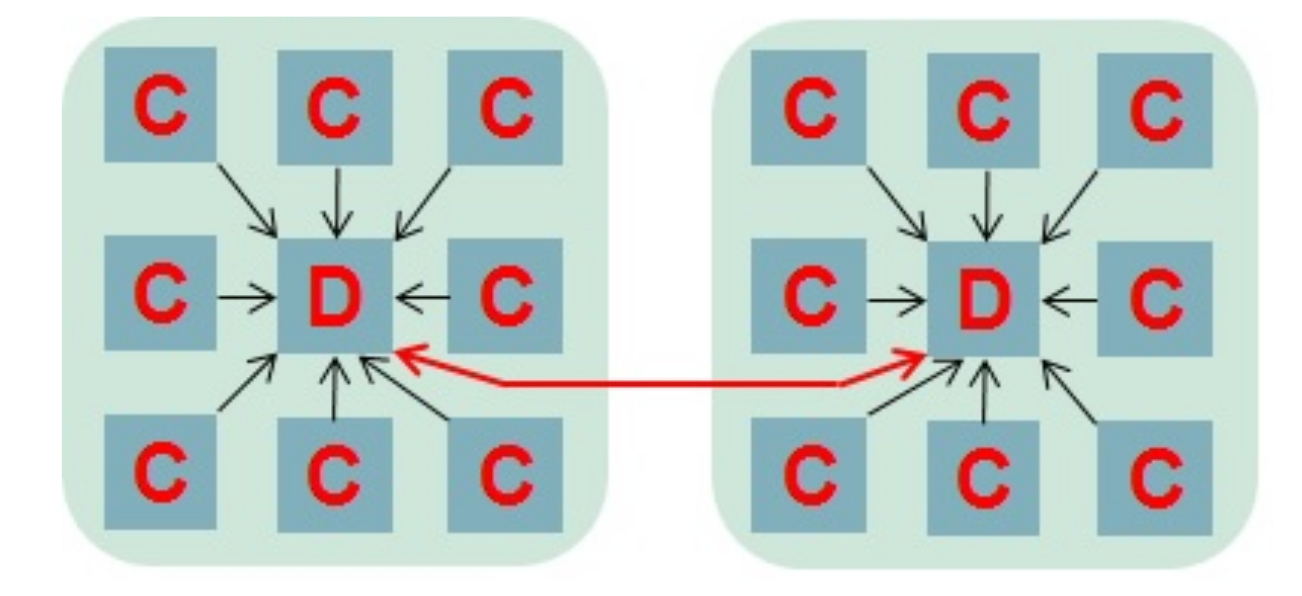
\includegraphics[scale=0.25]{MONC_to_IOserver_fig.png}
\caption{Schematic of the IO server to MONC computational core communication.
{\bf{C}} represent MONC computational cores and {\bf{D}} represents a data analytics
core, which is an IO server.}
\label{fig:ioserver}
\end{figure}

In order to overcome this data analytics bottle-neck, MONC uses a bespoke IO
server where some of the compute processes are dedicated
to handling the diagnostic and IO, rather than running the model. Typically one
or more cores in a processor will run the IO server and serve the remaining MONC
computational cores, which ''fire and forget'' their prognostic values.
This is illustrated in Figure~\ref{fig:ioserver}, where MONC computational
cores in a processor communicate values to their local IO server core. The IO
servers cores perform the diagnostic calculations, e.g. determining temporal and
spatial averaged values. Then the IO servers communicate amongst themselves with
limited amounts of data. Arranging the MONC compute cores and the IO server cores
in this fashion means that communications between MONC and the IO server are
local and typically performed in memory (and the same NUMA region) rather than
using the network. The ratio of IO servers to computational cores can be increased
for memory reasons but it is recommended that IO servers only serve MONC compute cores
that are available locally. For example, on the CRAY XC-40 architecture, i.e.
ARCHER and MONSOON, it is recommended  to use 11 or 8 MONC computational cores
for every 1 IO server core, so that there are 3 or 4 IO servers per core and
33 or 32 monc compute processes.

\subsection{IO server architecture}

Figure~\ref{fig:ioserver_workflow} shows the workflow of the IO server.
Data enters the IO server from a MONC computational core via the external API. In
MONC this API is the component \emph{IO\_bridge}, which sends data over as and
when it is needed/requested by the IO server depending on the XML IO configuraiton
(next section). The \emph{IO\_bridge} also registers with the IO server at model
start up and communicates specifics about the simulation, such as which fields
are registered, data sizes and simensions. The IO server is split into
two federators which contain the majority of the functionality of the MONC IO
server.

\subsubsection{Diagnostics federator}

The diagnostics federator (io/src/diagnostics/diagnostic\_federator.F90) is
responsible for data analytics. Depending on the IO configuration
defined in the users XML file, the diagnostics federator performs different
operations on raw fields received from a MONC computational core.
There are two main activities here
\begin{itemize}
  \item {Executing IO operators, e.g. maths, splitting of fields}
  \item {Perform the global communication, e.g. broadcast, reductions}
\end{itemize}
The communications pose a challenge as these should be implemented as collectives,
operations, e.g. a global reduction, but with MPI the order that collectives
are issued matters. As result an active messaging approach is required, where
messages (forming a broadcast, reduction etc) are asynchronously sent with a
unique identifier and the thread then performs some other activity. When and if
a corresponding message relating to this activity is returned (such as the result
of the reduction) then a thread is reactivated and the original action involved
a callback function which will be called to handle that message. The
asynchronicity adds significant complexity to the code and IO, but this is abstracted
in the communication routines and does allow for very
asynchronous issuing of dat. This is important and required
since the variable timestep in MONC means that the timing of the data sends
is non-deterministic.

\begin{figure}
  \centering
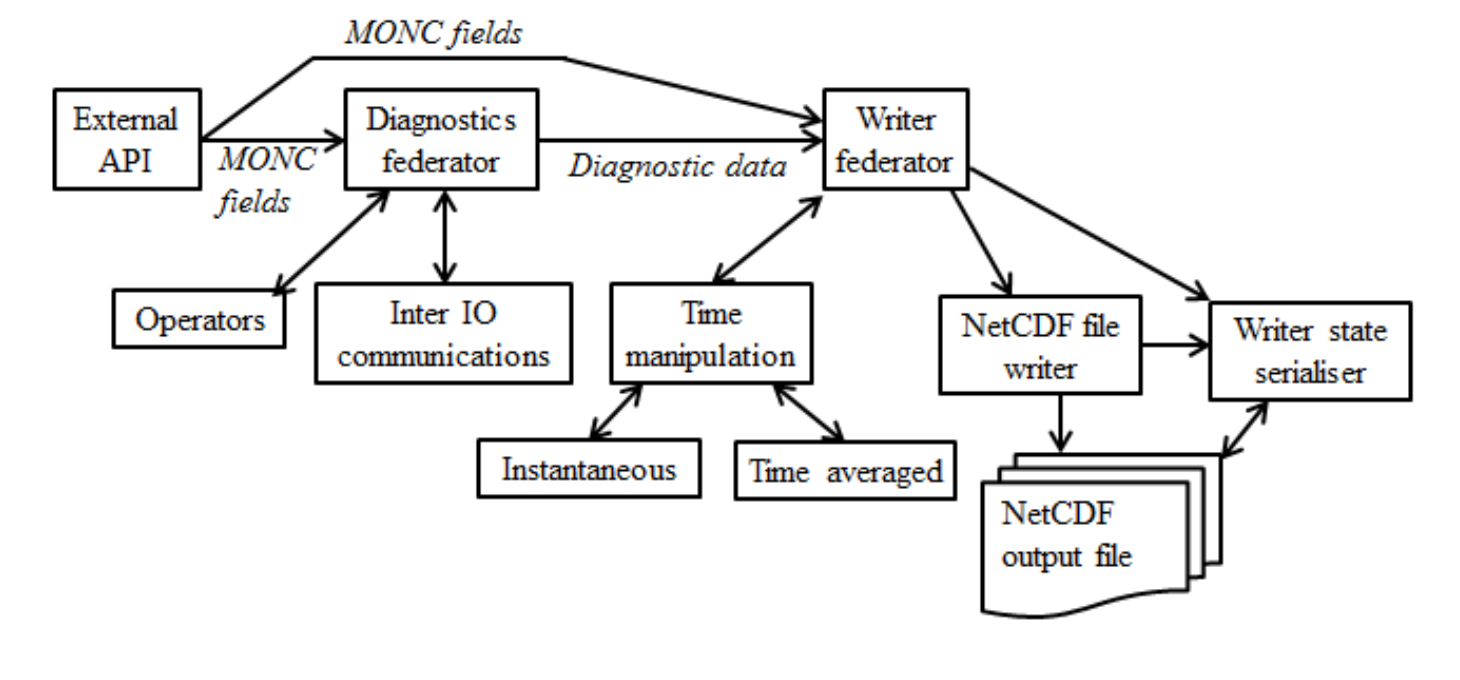
\includegraphics[scale=0.3]{IOserver_architecture_workflow.png}
\caption{Schematic of the IO server to workflow once data has been sent from MONC}
\label{fig:ioserver_workflow}
\end{figure}

\subsubsection{Write federator}

The write federator (io/src/writers/writer\_federator.F90) looks after
writing to file, in terms of defining files, writing to files and performing
time manipulation of fields as required by the user XML file. When data arrives,
either diagnostics or raw prognostics, it first goes through the writer field
manager (io/src/writers/writer\_field\_manager.F90), which enforces field
ordering. Due to the asynchronicity of the diagnostics federator, fields can
arrive out of order, i.e. timestep n+1 before n. The field manager will track
what fields have arrived and when, if there is a missing field it will queue
later data until the preceding field arrives when it can then fire them all to
the federator.

The federator will first perform time manipulation on the fields,
as defined by the user XML file. This manipulation may or may not produce a
value. If it does, it will check whether the value should trigger a write, i.e.
has the preconfigured time elapsed or not. If no write is to be performed then
the value is stored, otherwise the appropriate NetCDF file is defined and
writing of available fields will start.

In NetCDF file definition and creation is a collective, so all IO servers must
take part in this. Fields are then written and the file is closed once all
fields are written. Each IO server will register a callback to file closing
and the thread will then go idle, this again builds on the active messaging of
the diagnostics federator and, because closing a file is collective, all IO
servers will perform it at the same time as determined by the active messaging
synchronisation.

Finally closing a file is more complex than just calling the appropriate
NetCDF close function because other collective activities are also performed
here. Raw (prognostic) fields are written here because, for performance, we set
these as collective writes. Even though there are contributions from each local
computational MONC core, these are combined, based on relative location in
global domain, into as large as possible parcels of data which are then written.
During this an initialisation communication occurs to inform the IO servers
the maximum number of (non-contiguous) writes. Due to the collective nature, any IO
server that does not have this maximum number will just fill out the remainder
with empty writes. Storing the state of the IO server also occurs during the
file close stage. Due to the asynchronicity we wait for all the diagnostic
federator activities to complete and then checkpoint the state of the writer federator
and its associated activities.

\subsection{IO server configuration}

The IO server is configured in two places

\begin{itemize}
  \item {MONC User configuration file (\emph{.mcf}) - defines the
  IO server configuration file and some basic IO server parameters}
  \item {IO server configuration file (\emph{.xml} file) - defines the fields
  that are requested for diagnostics, the operations and the diagnostic write}
\end{itemize}

\subsubsection{MONC IO server configuration}
The IO server is switched on by turning on the \emph{iobridge} component in
the user configuration file, i.e.
\begin{lstlisting}
  iobridge_enabled=.true.
\end{lstlisting}
By default \emph{iobridge\_enabled=.false.} in the global\_config, so
it needs to be switched on in all user configuration files unless a user does
not require the IO server.

\begin{table}[H]
  \protect\caption{Configuration options to perform basic IO server set-up}
\label{tab:monc_io_config}
\begin{tabular}{|c|c|p{5cm}|p{3cm}|}
\hline
Configuration variable & configuration & description & global\_config \tabularnewline
name & type & & setting \tabularnewline
\hline
\multicolumn{4}{|c|}{\bf{Global configuration options}} \tabularnewline
\hline
   ioserver\_configuration\_file & string & path to the XML IO  & "io/description.xml" \tabularnewline
   &  & configuration file &  \tabularnewline
\hline
   moncs\_per\_io\_server & integer & Number of MONC compute processes & 3 \tabularnewline
    &   & for each IO server &  \tabularnewline
\hline
    enable\_io\_server & logical & If true the IO server is switched  & .true. \tabularnewline
   &  & on in the \emph{iobridge} & \tabularnewline
\hline
\multicolumn{4}{|c|}{\bf{Example of options that MUST be supplied in user configuration file}} \tabularnewline
\hline
  sampling\_frequency & integer & Number of timesteps between diagnostics & \emph{no default} \tabularnewline
    &  & or prognostics being sent from MONC to IO server & \tabularnewline
\hline
   \emph{mm} & float & output time interval for a diagnostic & \emph{no default} \tabularnewline
    &  & (this must be larger than model timestep $\times$ sampling\_frequency) & \tabularnewline
\hline
   diag\_write\_freq & float & time interval for diagnostic file writes & \emph{no default} \tabularnewline
 &  & (this must be larger that \emph{mm})  & \tabularnewline
\hline
\hline
\end{tabular}
\end{table}

Table~\ref{tab:monc_io_config} defines the globally available configuration options
required to set-up the IO server as well as some options, which are not present in the
global\_config but must be provided by the user. The global\_config options
include the ioserver\_configuration\_file, which is the top-level XML IO configuration
file. Examples of these files can be found in io/io\_cgf\_files/, e.g.
data\_write\_1file.xml. The set-up and contents of these files are discussed
in greater detail in the next section, but these files contain the XML for the requested
diagnostics, the MPI operators, diagnostics operators and the output frequency.
moncs\_per\_io\_server defines the number of MONC computational cores for
each IO server core. It is recommended that

\begin{itemize}
   \item {There are always more MONC cores tha IO server cores, so that the number
   of cores is maximised for computation.}
   \item {The IO servers only serve the cores on the local node, i.e. on ARCHER
   there are 24 cores per node. If moncs\_per\_io\_server=11, there will be
   22 MONC compute cores and 2 IO servers, which is on 1 node. If, however,
   moncs\_per\_io\_server=12, then there will be 2 IO servers still but 1
   will be serving a core on another node. This will be computationally inefficient
   at best but in reality, will probably fail.}
\end{itemize}

The configuration options in Table~\ref{tab:monc_io_config}, which have no default
in the global\_config relate to options that are parsed to the XML IO server
configuration file. These variables have no default configuration since they can
basically take any name as long as it is consistent with the option name in the
XML file. While the options can take any name, the function is as defined in
Table~\ref{tab:monc_io_config}. For example, the code block below shows an example
of the IO server configuration, in which there are 2 sampling\_frequency defined
and there are two time intervals for the output times defined, i.e. \emph{mm} and
\emph{mm1}. These values are parsed into the IO server through the XML file and
they control the diagostic transfer from MONC to the IO server, the output of
diagnostics and finally the time when to write diagnostics to file.
\begin{lstlisting}[caption={Example of the IO server configuration, taken from
  testcases/radiative\_convective\_equilibrium/RCE\_MO\_cray.mcf}]
  # IO server configuration
  ioserver_configuration_file="io/io_cfg_files/data_write_1file.xml"
  moncs_per_io_server=11
  sampling_frequency=20
  3d_sampling_frequency=100
  mm=3600.
  mm1=60.
  diag_write_freq=10800.
\end{lstlisting}
In general, it is recommended that the sampling of frequency of 3-D fields should not
be that small, i.e. greater than 50 depending on the required diagnostic output
and timestep. If it is too low, data will flood the system network, which will eventually
slow MONC and may cause MONC to crash.

\subsubsection{IO server configuration file (.xml)}

As well as the basic IO server configuration in the user configuration file,
the IO server is also configured using a structured XML configuration file such that the
IO server instructs its MONC processes about the specific type of data required
and when. Generic actions for handling this data are included with the IO server,
which can be added to if required, and are configured in a high level fashion by
the user via the IO server XML configuration file.

The IO server configuration file is provided by the user configuration file, i.e.
\begin{lstlisting}
  # IO server configuration
  ioserver_configuration_file="io/io_cfg_files/data_write_1file.xml"
\end{lstlisting}

This file either contains or links to other .xml files that contain 4 important
sections
\begin{itemize}
  \item {{\bf{Data definition}} - This defines the data that the IO server will
  receive from MONC and can contain many fields, e.g. see
  io/io\_cfg\_files/profiles.xml or io/io\_cfg\_files/scalars.xml
  (note that these files are "\#include" in the ioserver\_configuration\_file).
  More generally, the examples below present two fields, \emph{a} and \emph{b}.
  \emph{a} is defined as an array of doubles that are optional, i.e. MONC will
  only send this over if the variabel is available. The field b is an integer
  scalar, where \emph{optional} is ommitted, so this is \emph{b} is mandatory,
  i.e. if MONC is not able to send it then an error is raised.) This specific
  data definition is sent from MONC every \{sampling\_frequency\}, where the
  sampling\_frequency is defined in the user configuration file ( the \{ \}
  braces do this substitution.)
  \begin{lstlisting}
  <data-definition name="flux_fields" frequency="{sampling_frequency}">
  	<field name="a" type="array" data_type="double" optional=true/>
  	<field name="b" type="scalar" data_type="integer"/>
  </data-definition>
  \end{lstlisting}
  }
  \item{{\bf{Data handling}} - This sections defines any processing or analysis
  of the data once the IO server has received it from their
  respective MONCs. For example, the code block below shows a snippet from
  scalars.xml. In this example the required diagnostic is a domain
  mean vapour water path. The field, \emph{vwp} is a 2-D horizontal slice field,
  which is passed from MONC component scalar\_diagnostics.F90, to the IO
  server. The first operation is to perform a local reduction and a sum of the
  field. This is then followed a global sum (and reduction), which results in
  \emph{VWP\_mean\_g}. Finally, an equation is applied to \emph{VWP\_mean\_g}
  to derive the global mean, i.e.
  \emph{VWP\_mean}.
  \begin{lstlisting}
  <data-handling namespace="scalar_fields">
    <diagnostic field="VWP_mean"  type="scalar" data_type="double" units="kg/m^2">
	    <operator name="arithmetic" result="VWP_mean" equation="VWP_mean_g/({x_size}*{y_size})"/>
	    <communication name="reduction" operator="sum" result="VWP_mean_g" field="VWP_mean_loc_reduced" root="auto"/>
	    <operator name="localreduce" operator="sum" result="VWP_mean_loc_reduced" field="vwp"/>
    </diagnostic>
  \end{lstlisting}
  }
  \item{{\bf{Group}} - It is useful to group fields together and then refer to
  the group rather than individual fields. The section provides a way of doing
  this. For example, the code block below shows a snippet from
  \emph{scalars.xml}
  \begin{lstlisting}
  <group name="scalar_timeseries" namespace="scalar_fields">
    <member name="VWP_mean"/>
    <member name="LWP_mean"/>
  \end{lstlisting}
  This group definition is very simple, but there is the stipulation that a
  field should not appear twice in the same group.
  }
  \item {{\bf{Data writing}} - This sections defines what is written to the netcdf
  file. For example, the code block below shows that fields will write to
  file \emph{diagostics\_ts.nc}, at the time \emph{diag\_write\_freq}, which comes
  from the \emph{user\_config.mcf}. This code block also includes the groups
  with a time\_manipulation, i.e. averaged, which is averaged over time, or
  instantaneous. Finally, the the write section includes the \emph{output\_frequency},
  which relates to time defined in the user configuration file. Thus, this section
  includes most of the links to the IO confguration in user configuration file.
  \begin{lstlisting}
  <data-writing>
    <file name="diagnostic_files/diagnostics_ts.nc" write_time_frequency="{diag_write_freq}" title="All diagnostic values">
      <include group="profile_timeseries" time_manipulation="averaged" output_frequency="{mm}"/>
      <include group="scalar_timeseries" time_manipulation="instantaneous" output_frequency="{mm1}"/>
      <include group="3d_fields" time_manipulation="instantaneous" output_frequency="{mm}"/>
      <include group="2d_fields" time_manipulation="instantaneous" output_frequency="{mm}"/>
    </file>
  </data-writing>
  \end{lstlisting}
  }
\end{itemize}

This section has presented an overview of the XML config. There are many more
operators and functions that can be used in the IO server. These are documented
on the {\href{https://code.metoffice.gov.uk/trac/monc/wiki/MoncDoc/Diagnostics}
{MONC diagnostics wiki}} and users should refer to that for further information.

\section{Diagnostics}

There are a significant number of diagnostics available in MONC. These diagnostics
fall into four categories
\begin{itemize}
  \item {3-D fields}
  \item {2-D fields}
  \item {1-D vertical profile fields}
  \item {Scalar fields}
\end{itemize}
All diagnostics are output as timeseries with an output
timestep determined by the output time interval for a diagnostic (see
Table~\ref{tab:monc_io_config}, \emph{mm}). The naming convention for the
diagnostic categories relates the number of spatial dimensions.

The previous section discussed the IO server and IO server configuration, which
ultimately generates, finalises and writes these diagnostics to a netcdf file.
In many cases, the MONC diagnostic system needs the MONC side generation of
published fields for the the IO server. There are 2 broad options for publishing fields
to the IO server
\begin{enumerate}
  \item {Send 3-D prognostic fields directly to the IO server}
  \item {Perform some diagnostic calculation on the MONC side to derive the fields
  to send to the IO server}
\end{enumerate}
(1) is the simplest method and requires little or no extra code on the MONC side, since
the model prognostics (u,v,w,th,q) are available through the \emph{iobridge}.
In the IO server there are operators that can diagnose some quantities from these
prognostic fields. Users can also write their own operators to work on the
prognostic fields - see \url{https://code.metoffice.gov.uk/trac/monc/wiki/MoncDoc/Diagnostics}
for some details. Although these IO operators exist, care needs to be taken
when using only prognostic fields and performing all diagnostic calculation on
the IO server since sending 3-D prognostic data at regular time intervals
can result in a significant data loading and buffering on the
HPC network, which in turn can stall or stop MONC. As a result, it is recommended
that 3-D prognostics fields are only sent to the IO server to be written to file.

Option (2) avoids some of the data buffering issues because published fields are
diagnosed over the local decomposition on the MONC side, which reduces the data
to send. These diagnosed published fields can then be sent to the IO server on
request, where the IO server can perform mainly the global communication
operations, which would stall MONC compute if performed on the MONC side.

Diagnostics can be derived during the MONC compute from either specific
diagnostics component, e.g. \emph{profiles\_diagnostics} and
\emph{scalar\_diagnostics}, or directly from a science component, e.g. the
radiative fluxes and heating rates in \emph{socrates\_couple}. When including
new diagnostics, it is recommended that the diagnostics do not use modules from
other science components to re-derive variables, since this will break the
independence of the component architecture. If variables from other science
components are required, we recommend that the fields are added into the
current\_state in the model\_core (Note: there are places in MONC components
where this recommendation is not adhered to).

The following sections will go into more detail about the MONC diagnostic
categories and, where appropriate present examples or link to code to help adding
diagnostics.

\subsection{3-D diagnostics}

There are two types of 3-D diagnostics that can be output

\begin{itemize}
  \item {A 3-D diagnostic from a field that exists in current\_state, e.g.
  prognostic fields}
  \item {A 3-D diagnostic from that needs to be derived from fields in current\_state}
\end{itemize}

\subsubsection{Including 3-D diagnostic from current\_state}

If a field already exists in current\_state then outputting the field as a
diagnostic only requires additions to the \emph{iobridge} and the addition of
the IO configuration to an XML IO configuration file. For example, to add a
3-D diagnostic for the diffusion coefficient (current\_state\%diffusion\_coefficient)
add the following to the \emph{iobridge} component
\begin{enumerate}
  \item {Define the array size of the field being sent
  to the IO server and assign a diagnostic name to this space, i.e. diff:
  \begin{lstlisting}
    if (is_component_enabled(current_state%options_database, "diffusion")) then
      raw_generic=>generate_sendable_description(z_size, y_size, x_size)
      call c_put_generic(sendable_fields, "diff", raw_generic, .false.)
    endif
  \end{lstlisting}
  where the condition is specific to the diffusion coefficient. If adding other
  3-D diagnostics, e.g. absolute temperature, this condition needs to modified
  to represent the appropriate dependency.
  }
  \item {Send the diffusion field, i.e.
  current\_state\%diff\_coefficient to the IO server using the
  pack\_prognostic\_flow\_field function:
  \begin{lstlisting}
    else if (field%name .eq. "diff") then
      pack_array_into_send_buffer=pack_prognostic_flow_field(
        data_definition%send_buffer, &
        current_state%diff_coefficient, current_buffer_point, &
        current_state%local_grid)
  \end{lstlisting}
  where field\%name must be the as the same as the diagnostic name, i.e. second
  argument in call c\_put\_generic in (1). pack\_prognostic\_flow\_field sends the
  local decomposition of the domain, which is the domain on each processor once
  the model domain has been decomposed.
  }
\end{enumerate}

Then in order to combine all the local decompositions and output 3-D fields,
add the following to the XML IO configuration file (io/io\_cfg\_files/3d\_fields.xml)
\begin{enumerate}
  \item {In the data-definition section add
  \begin{lstlisting}
     <field name="diff" type="array" data_type="double" size="z,y,x" collective=true optional=true/>
  \end{lstlisting}
  }
  \item {In the group section add
  \begin{lstlisting}
    <member name="diff"/>
  \end{lstlisting}
  }
\end{enumerate}
While the above makes the IO configuration changes in io/io\_cfg\_files/3d\_fields.xml,
you are free to develop separate IO configuration files for your new diagnostics.
If you do this you must remember to include the group, e.g. "3d\_fields" in the
data-writing statement, e.g. see io/io\_cfg\_files/data\_write\_1file.xml.

\subsubsection{Deriving 3-D diagnostic from current\_state}

There are many scenarios when a diagnostic needs to be derived from fields in
current\_state and then output. For example, absolute temperature is a useful
diagnostic but it is not a prognostic field in MONC and hence is not stored in
current\_state. When you need to output a 3-D diagnostic such as absolute
temperature, it needs to be (i) derived from variables in current\_state, i.e. thref
and th, and (ii) published to the IO server using
the field\_value\_retrieval\_callback and field\_information\_retrieval\_callback.
Below are the steps required to output 3-D absolute temperature using the
\emph{test} component (defined in section 3) as an example
\begin{enumerate}
  \item {Add pointers for field\_value\_retrieval\_callback and
  field\_information\_retrieval\_callback to the \emph{test} component
  descriptor, e.g.
  \begin{lstlisting}
  type(component_descriptor_type) function test_get_descriptor()
   test_get_descriptor%name="test_component"
   test_get_descriptor%version=0.1
   test_get_descriptor%initialisation=>initialisation_callback
   test_get_descriptor%timestep=>timestep_callback
   test_get_descriptor%field_value_retrieval=>field_value_retrieval_callback
   test_get_descriptor%field_information_retrieval=> &
                                   field_information_retrieval_callback

   allocate(test_get_descriptor%published_fields(1))

   test_get_descriptor%published_fields(1)="absolute_T"

  end function test_get_descriptor
  \end{lstlisting}
  where "allocate(test\_get\_descriptor\%published\_fields(1))" is the number of
  fields that will be published from the component, i.e. number of fields
  available to the IO server. "test\_get\_descriptor\%published\_fields(1)="absolute\_T""
  is the name of the published field. This name is the identifier in the IO
  server, and must be the same as the name in the "data-definition" section in
  IO configuration file.
  }
  \item {Allocate the 3-D field to be derived this \emph{test} and used as the
  diagnostic:
  \begin{lstlisting}
  if (current_state%th%active) then
   allocate(TdegK(current_state%local_grid%size(Z_INDEX),  &
   current_state%local_grid%size(Y_INDEX),            &
   current_state%local_grid%size(X_INDEX)))
  endif
  \end{lstlisting}
  "TdegK" is the array used in MONC to derive absolute temperature. It is allocated
   using the current\_state\%local\_grid to ensure the array is sized for the local
   decomposition (not the global grid).
   }
   \item{Derive the 3-D field in \emph{test} using the following
   \begin{lstlisting}
     integer :: current_y_index, current_x_index, target_x_index, target_y_index

     if (current_state%halo_column) return

     current_y_index=current_state%column_local_y
     current_x_index=current_state%column_local_x
     target_y_index=current_y_index-current_state%local_grid%halo_size(Y_INDEX)
     target_x_index=current_x_index-current_state%local_grid%halo_size(X_INDEX)

     if (current_state%th%active) then
       TdegK(:,target_y_index, target_x_index) =                            &
            (current_state%th%data(:,current_y_index,current_x_index)       &
            + current_state%global_grid%configuration%vertical%thref(:)     &
            * current_state%global_grid%configuration%vertical%rprefrcp(:))
     endif
   \end{lstlisting}
   It is important to note that there is current\_index - used on the right-hand-side,
   which is the actual array index of the variable, and a target\_index - on the
   left hand side. This is the index with the halos subtracted. The target\index
   is used so that diagnostic does not include halos.
   }
   \item{Add the field\_value\_retrieval\_callback and
   field\_information\_retrieval\_callback to the component, e.g.
   \begin{lstlisting}
   subroutine field_information_retrieval_callback(current_state, name, field_information)
     type(model_state_type), target, intent(inout) :: current_state
     character(len=*), intent(in) :: name
     type(component_field_information_type), intent(out) :: field_information
     field_information%field_type=COMPONENT_ARRAY_FIELD_TYPE
     field_information%number_dimensions=3
     field_information%dimension_sizes(1)=current_state%local_grid%size(Z_INDEX)
     field_information%dimension_sizes(2)=current_state%local_grid%size(Y_INDEX)
     field_information%dimension_sizes(3)=current_state%local_grid%size(X_INDEX)
     field_information%data_type=COMPONENT_DOUBLE_DATA_TYPE
     if (name .eq. "absolute_T") then
        field_information%enabled=current_state%th%active
     else
        field_information%enabled=.true.
     endif
   end subroutine field_information_retrieval_callback

   subroutine field_value_retrieval_callback(current_state, name, field_value)
     type(model_state_type), target, intent(inout) :: current_state
     character(len=*), intent(in) :: name
     type(component_field_value_type), intent(out) :: field_value

     integer :: k
     if (name .eq. "absolute_T") then
        allocate(field_value%real_3d_array(current_state%local_grid%size(Z_INDEX),  &
             current_state%local_grid%size(Y_INDEX),                                &
             current_state%local_grid%size(X_INDEX)))
        field_value%real_3d_array(:,:,:) = TdegK(:,:,:)
     end if

   end subroutine field_value_retrieval_callback
   \end{lstlisting}
   It can be seen that the field\_information\_retrieval\_callback determines the
   the dimensions of the diagnostic and whether it is required, while the
   field\_value\_retrieval\_callback applies the derived field, "TdegK", to the
   "field\_value" structure, which is available for the IO server.
   }
   \item{The final stage is to add "absolute\_T" to the XML IO configuration file
   e.g
   \begin{lstlisting}
   <data-definition name="3d_fields_data" frequency="{sampling_frequency}">
     <field name="absolute_T" type="array" data_type="double" size="z,y,x"
                                                collective=true optional=true/>
   </data-definition>

  <group name="3d_fields">
   <member name="absolute_T"/>
  </group>
   \end{lstlisting}}
\end{enumerate}

\subsection{2-D fields and scalar fields}

In general all 2D diagnostics need to be derived on the MONC side, e.g.
liquid water path and surface precipitation. For a full understanding
 about how to calculate and output 2-D diagnostics, the user should go through
the \emph{scalar\_diagnostics} component, which derives a wide range of
2-D fields. Here we will step through what needs
to be included to add liquid water path (lwp) and vapour water path (vwp)
\begin{enumerate}
  \item {
  In a similar fashion to
  the 3-D fields, in order to publish 2-D diagnostic fields to the IO server, the first
  stage is to add pointers for field\_value\_retrieval\_callback and
  field\_information\_retrieval\_callback and allocate the published field e.g.

  \newpage

  \begin{lstlisting}[caption={code snippet from scalar\_diagnostics, which
    shows the allocation of water path published fields}]
  scalar_diagnostics_get_descriptor%field_value_retrieval=> &
                                            field_value_retrieval_callback
  scalar_diagnostics_get_descriptor%field_information_retrieval=> &
                                            field_information_retrieval_callback
  allocate(scalar_diagnostics_get_descriptor%published_fields(16))
  scalar_diagnostics_get_descriptor%published_fields(1)="vwp"
  scalar_diagnostics_get_descriptor%published_fields(2)="lwp"
  \end{lstlisting}
  }
  \item{allocate the 2-D field to be derived, e.g.
  \begin{lstlisting}
  allocate(vwp(y_size_local, x_size_local), lwp(y_size_local, x_size_local), &
  \end{lstlisting}
  It is important to note that the fields are declared using the local
  domain size, not the global domain. This further demonstrates that any
  diagnostic derived on the MONC side must be confined to the local decomposition.
  }
  \item{Add the code required to derive the lwp and vwp, e.g.
  \begin{lstlisting}
  do k = 2, current_state%local_grid%size(Z_INDEX)
     vwp(target_y_index, target_x_index)=vwp(target_y_index, target_x_index) &
          +dz_rhon_fac(k)* &
          current_state%q(current_state%water_vapour_mixing_ratio_index)%data(k, &
          current_y_index, current_x_index)
     lwp(target_y_index, target_x_index)=lwp(target_y_index, target_x_index) &
          +dz_rhon_fac(k)* &
          current_state%q(current_state%liquid_water_mixing_ratio_index)%data(k, &
          current_y_index, current_x_index)
  enddo
  \end{lstlisting}
  In the code snippet above, both vwp and lwp are integrated over altitude to
  give a value for each column.
  }
  \item{
  Then the dimensions of the field to send are defined in
  field\_information\_retrieval\_callback and the field is sent using
  the following code in field\_value\_retrieval\_callback
  \begin{lstlisting}
  else if (name .eq. "vwp") then
     allocate(field_value%real_2d_array(current_state%local_grid%size(Y_INDEX), &
         current_state%local_grid%size(X_INDEX)))
     field_value%real_2d_array(:,:)=vwp(:,:)
  else if (name .eq. "lwp") then
     allocate(field_value%real_2d_array(current_state%local_grid%size(Y_INDEX), &
         current_state%local_grid%size(X_INDEX)))
     field_value%real_2d_array(:,:)=lwp(:,:)
  \end{lstlisting}
  Since the field being sent is 2-D the field is written to
  field\_value\%real\_2d\_array
  }
\end{enumerate}

The 2-D fields are then used as the direct output for 2-D diagnostics (see
io/io\_cfg\_files/2d\_fields.xml). They are also used for the input to the
scalar diagnostics (io/io\_cfg\_files/scalar\_fields.xml), where the IO configuration
is used to derive domain means, minimum and maximum of the 2-D field. The
focus of this subsection has been the \emph{scalar\_diagnostics} component, since
most of the 2D and scalar diagnostics are derived from there. It is important
to note that in addition, 2-D diagnostic for surface precipitation is derived in
\emph{casim}, while the surface and top-of-atmosphere radiation fluxes are derived
in \emph{socrates\_couple}.

\subsection{1-D profile diagnostics}

1-D profile diagnostics generally represent horizontally averaged vertical
profiles. These fields are derived in the \emph{profile\_diagnostics},
\emph{subgrid\_profile\_diagnostics} and \emph{flux\_budgets} components. Although,
these components produce very different diagnostics, when it deriving a published
field the components employ very similar methods, i.e. include
field\_information\_retrieval\_callback and field\_value\_retrieval\_callback,
allocate the published field, allocate the fields to derive, perform the derivation
and send the derived field. The code for this is very similar to the already
presented for the 3-D and 2-D fields. An important difference to mention, is that
no horizontal averaging is performed on the MONC side. Instead, the MONC side
performs the local totalling of the profiles on the local decomposition, which
are sent to the IO server. The IO server performs the global total and the
averaging occurs then (for a code example see \emph{profile\_diagnostics} and
follow the variable u\_wind\_tot, then view the same variable in
io/io\_cfg\_files/profile\_fields.xml). While this may seem complicated, this
ensures that mean calculations are reproducible for different decompositions.

\section{Checkpoint restart and continuation runs}

An important technical aspect of MONC is the ability for it to perform checkpoint
restarts. This is important for 2 reasons

\begin{itemize}
  \item {HPCs often limit the wallclock time available for a simulation, e.g.
   on MONSOON the wallclock is limited to 3 hours. For almost all applications
   simulations will take longer than 3 hours wallclock time, so there needs to
   be a method to stop a simulation (checkpoint) and the restart from that point}
  \item {It is often useful to break a long integration into smaller integrations
  with regular model dumps, so that if something occurs to stop the simulation
  unexepectedely, it does not need to be run from the beginning}
\end{itemize}

In MONC, checkpointing involves saving the state of MONC computation and state
of the IO server (diagnostics state) at a configured time or number of timesteps.
Given the need to dump the state of the IO server, it is preferable to perform
the checkpoint restart via the IO server. Checkpoint restarts can be performed
without the IO server, but, it is important to note, that this will mean no diagnostics
are dumped and so it is assumed that diagnostics are not required. In this section
we will only discuss checkpoint restart via IO server.

In order to use checkpoint restarts via the IO server, it is first
necessary to enable the checkpointer component and the IO server, i.e. in the
user configuration file the following must be set
\begin{lstlisting}
  checkpointer_enabled=.true.
  iobridge_enabled=.true.
\end{lstlisting}

The \emph{checkpointer} component, which is enabled by default in global\_config,
reads the current state of the model with-respect-to computation and supports
checkpoint restart during MONC computation. This component will also
write out the state of the MONC computation but not the diagnostics state. This
will mean that diagnostics will start from fresh at restart, which is no use if
means are being performed over the checkpoint. To overcome this, the IO
server is used, by enabling \emph{iobridge} in the user configuration file and
including the following line in the XML IO server configuration file

\begin{lstlisting}[caption={Snippet of XML IO server configuration for
  checkpoint restarting from the IO server. Taken from
  io/io\_cfg\_files/data\_write\_1file.xml}]
  #include "io/io_cfg_files/checkpoint.xml"
\end{lstlisting}

io/io\_cfg\_files/checkpoint.xml is an XML IO server configuration file,
which defines all the MONC fields that need to be
dumped to store the MONC computational and IO
state, which enables no break in the collection of diagnostics and the averaging
of fields during a checkpoint restart.

\subsection{MONC configuration for checkpoint restart}

Table~\ref{tab:monc_checkpoint_config} presents the configuration options
for setting up checkpoint restart, while the code snippet below presents a
an example configuration from the RCE case. In this example,
the checkpoint\_frequency is set to 0. This will cause
MONC to perform a model dump and a stop, when the simulation has reached the
MONC walltime\_limit of "00:40:00", which is 40 minutes of wall clock time.
If the checkpoint\_frequency is greater than 0 then this represents
the number of model timesteps to complete in between model dumps. It is recommended
that all users employ a checkpoint\_frequency of 0 and make sure the the walltime\_limit
is lower than the machine wall-time limit (see next section). check\_walltime\_frequency
is the number of timesteps that MONC will check the wall-clock time. This check involves
global operation, since all processors have to synchronise, so it is recommended
that this frequency is not too low, i.e. around 100 works well.

\begin{lstlisting}[caption={Snippet of the MONC configuration for
  checkpoint restarting. Taken from
  testcases/radiative\_convective\_equilibrium/RCE\_MO\_cray.mcf}]
  # Checkpoint configuration
  checkpoint_frequency=0
  checkpoint_file="checkpoint_files/RCE_dump.nc"
  check_walltime_frequency=10
  walltime_limit=00:40:00
\end{lstlisting}

\begin{table}[H]
  \protect\caption{Configuration options to perform checkpoint restart}
\label{tab:monc_checkpoint_config}
\begin{tabular}{|c|c|p{5cm}|p{3cm}|}
\hline
Configuration variable & configuration & description & global\_config \tabularnewline
name & type & & setting \tabularnewline
\hline
   checkpoint\_frequency & integer & number of timesteps in between model dumps. If this is set to 0 then checkpoint will occur when walltime\_limit is reached & 10 \tabularnewline
\hline
   checkpoint\_file & string & name of the checkpoint file & 'monc.nc' \tabularnewline
\hline
  checkpoint\_unique\_per\_dump & logical & Only used when IO server is not enabled. If true all dump file will be saved  & .false. \tabularnewline
\hline
  walltime\_limit & string & Internal walltime limit for simulation time. & None \tabularnewline
\hline
   check\_walltime\_frequency & integer & number of model timesteps between checks for the wall-clock time & 200 \tabularnewline
\hline
\hline
\end{tabular}
\end{table}

\subsection{Restarting MONC from checkpoint file}

In order to start a simulation from a checkpoint file, the simulation is
executed with a reference to the the checkpoint file, rather than a
configuration file, e.g. using the previous snippet of checkpoint configuration,
a simulation could be restarted from checkpoint\_files/RCE\_dump.nc with
the following

\begin{lstlisting}
mpirun -np 2 ./build/bin/monc_driver.exe --checkpoint=checkpoint_files/RCE_dump.nc
\end{lstlisting}

Likewise if a simulation needs to be restarted using \emph{qsub}, then the
\emph{aprun} command in the \emph{.pbs} file needs to be changed from
\begin{lstlisting}
aprun -B ./build/bin/monc_driver.exe --config=$TESTCASE &> monc_stdout/output
\end{lstlisting}
to
\begin{lstlisting}
aprun -B ./build/bin/monc_driver.exe --checkpoint=$checkpoint_filename  &> monc_stdout/output
\end{lstlisting}
where \emph{checkpoint\_filename} is the path and filename for the checkpoint file.

When restarting the checkpoint component will read the optionsdatabase that is
stored in the checkpoint file and restart the simulation. If the user wants to
make a change to the simulation, e.g. change the frequency of diagnostic output,
the change to configuration is added in the command line. For example, the
code below shows the submission of a simulation with a change in the termination
time
\begin{lstlisting}
mpirun -np 2 ./build/bin/monc_driver.exe --checkpoint=checkpoint_files/RCE_dump.nc --termination_time=86400.0
\end{lstlisting}
It is important to note that at the time of writing, the original MONC
configuration file is not re-read during a restart, so any changes to that file
will have no impact. Changes must be added using command line options.

\subsection{Continuation runs}

So far in this section the method for performing a restart is highly manual, i.e.
MONC will do the checkpoint and produce a checkpoint file, then stop. The user must
then manually resubmit the job referencing the the checkpoint file. Ideally,
this should be an automated process.

As part of the MONC development, a continuation script and submission scripts
have been developed to facilitate automatic continuation runs on XC-40 systems
or systems that use the PBS scheduling system. The continuation script and an
example PBS script are on the MONC trunk, i.e. \emph{misc/continuation.sh} and
\emph{submonc.pbs}, respectively. The intention of these scripts are that, in
general a user should only need to change \emph{submonc.pbs} so that it includes
the appropriate settings. The code block below shows a snippet of the script
from \emph{submonc.pbs}
\begin{lstlisting}
export SUBMISSION_SCRIPT_NAME=submonc.pbs
export MONC_EXEC=./build/bin/monc_driver.exe

export TESTCASE=testcases/stable/Fog_Porson2011.mcf
export STDOUT_DIR=monc_stdout
export CP_DIR=checkpoint_files
export RUN_NAME=fog_dump_
\end{lstlisting}
\emph{submonc.pbs} is a bit fussy about changes. Hence,
if a user is changing the script the following needs to be correct
\begin{itemize}
  \item {SUBMISSION\_SCRIPT\_NAME must be the script file name. If the script name
   changes from \emph{submonc.pbs} this variable must be the same as the change,
   otherwise the submission script will not be located}
  \item {TESTCASE must be set to the configuration file that the user wants to
  simulate}
  \item {RUN\_NAME must be the name of the checkpoint\_file in the MONC
  configuration, with the ".nc" replaced by "\_". For example, the
  configuration for the checkpoint\_file in
  testcases/radiative\_convective\_equilibrium/RCE\_MO\_cray.mcf is
  \begin{lstlisting}
  checkpoint_file="checkpoint_files/RCE_dump.nc"
  \end{lstlisting}
  Thus, if a user is running this config as continuation run \emph{submonc.pbs}
  needs the following changed
  \begin{lstlisting}
  export RUN_NAME=RCE_dump_
  \end{lstlisting}
  }
\end{itemize}
It is important these changes are made for a continuation run to work, since
these changes inform the \emph{continuation.sh} which files it should run.

\section{Test-cases}



\appendix

\section{3-D diagnostic fields}

\begin{table}[H]
  \protect\caption{3-D diagnostic fields available in 3d\_fields.xml}
\label{tab:3d-fields}
\begin{tabular}{|c|p{7cm}|c|c|}
\hline
 Diagnostic name & Description & Units & LEM equivalent \tabularnewline
\hline
   w & vertical velocity & m s$^{-1}$ & W \tabularnewline
\hline
   u & horizontal velocity x-component & m s$^{-1}$ & U \tabularnewline
\hline
   v & horizontal velocity y-component & m s$^{-1}$ & V \tabularnewline
\hline
   th & potential temperature pertubation from the reference profile & K & TH \tabularnewline
\hline
   q & moisture fields (see Table~\ref{tab:3d-fields}) &  & Q.. \tabularnewline
\hline
\hline
\end{tabular}
\end{table}

\begin{table}[H]
  \protect\caption{3-D diagnostic q fields}
\label{tab:3d-fields}
\begin{tabular}{|c|p{7cm}|c|c|}
\hline
 Diagnostic name & Description & Units & LEM equivalent \tabularnewline
\hline
q\_vapour & water vapour mass mixing ratio & kg kg$^{-1}$ & Q01 \tabularnewline
\hline
q\_cloud\_liquid\_mass & cloud liquid mass mixing ratio & kg kg$^{-1}$ & Q02 \tabularnewline
\hline
q\_rain\_mass & rain mass mixing ratio & kg kg$^{-1}$ &  \tabularnewline
\hline
q\_ice\_mass & ice mass mixing ratio & kg kg$^{-1}$ &  \tabularnewline
\hline
q\_snow\_mass & snow mass mixing ratio & kg kg$^{-1}$ &  \tabularnewline
\hline
q\_graupel\_mass & graupel mass mixing ratio & kg kg$^{-1}$ &  \tabularnewline
\hline
q\_cloud\_liquid\_number & cloud drop number concentration & kg$^{-1}$ & \tabularnewline
\hline
q\_rain\_number & rain drop number concentration & kg$^{-1}$ & \tabularnewline
\hline
q\_ice\_number & ice number concentration & kg$^{-1}$ & \tabularnewline
\hline
q\_snow\_number & snow number concentration & kg$^{-1}$ & \tabularnewline
\hline
q\_graupel\_number & graupel number concentration & kg$^{-1}$ & \tabularnewline
\hline
q\_rain\_third\_moment & rain third moment &  & \tabularnewline
\hline
q\_snow\_third\_moment & snow third moment &  & \tabularnewline
\hline
q\_graupel\_third\_moment & graupel third moment &  & \tabularnewline
\hline
q\_aitken\_sol\_mass & aitken mode soluble aerosol mass mixing ratio & kg kg$^{-1}$ & \tabularnewline
\hline
q\_aitken\_sol\_number & aitken mode soluble aerosol number concentration & kg$^{-1}$ & \tabularnewline
\hline
q\_accum\_sol\_mass & accumulation mode soluble aerosol mass mixing ratio & kg kg$^{-1}$ & \tabularnewline
\hline
q\_accum\_sol\_number & accumulation mode soluble aerosol number concentration & kg$^{-1}$ & \tabularnewline
\hline
q\_coarse\_sol\_mass & coarse mode soluble aerosol mass mixing ratio & kg kg$^{-1}$ & \tabularnewline
\hline
q\_coarse\_sol\_number & coarse mode soluble aerosol number concentration & kg$^{-1}$ & \tabularnewline
\hline
q\_active\_sol\_liquid & activated soluble aerosol mass mixing ratio in cloud liquid & kg kg$^{-1}$ & \tabularnewline
\hline
q\_active\_sol\_rain & activated soluble aerosol mass mixing ratio in rain & kg kg$^{-1}$ & \tabularnewline
\hline
q\_coarse\_dust\_mass & coarse mode insoluble aerosol mass mixing ratio & kg kg$^{-1}$ & \tabularnewline
\hline
q\_coarse\_dust\_number & coarse mode insoluble aerosol number concentration & kg$^{-1}$ & \tabularnewline
\hline
q\_active\_insol\_ice & activated insoluble aerosol mass mixing ratio in ice & kg kg$^{-1}$ & \tabularnewline
\hline
q\_active\_sol\_ice & activated soluble aerosol mass mixing ratio in ice & kg kg$^{-1}$ & \tabularnewline
\hline
q\_active\_insol\_liquid & activated insoluble aerosol mass mixing ratio in cloud liquid & kg kg$^{-1}$ & \tabularnewline
\hline
q\_accum\_insol\_mass & accumulation mode insoluble aerosol mass mixing ratio & kg kg$^{-1}$ & \tabularnewline
\hline
q\_accum\_insol\_number & accumulation mode insoluble aerosol number concentration & kg$^{-1}$ & \tabularnewline
\hline
q\_active\_sol\_number & activated soluble aerosol number concentration & kg$^{-1}$ & \tabularnewline
\hline
q\_active\_insol\_number & activated insoluble aerosol number concentration & kg$^{-1}$ & \tabularnewline
\hline
\hline
\end{tabular}
\end{table}


\begin{thebibliography}{}
\item{Abel, S. J. and Shipway, B. J. (2007), A comparison of cloud-resolving model simulations of trade wind cumulus with aircraft observations taken during RICO. Q.J.R. Meteorol. Soc., 133: 781–794. doi: 10.1002/qj.55}

\item{Ackerman, A. S., vanZanten, M. C., Stevens, B., Savic-Jovcic, V., Bretherton, C. S., Chlond, A., Golaz, J-C., Jiang, H., Khairoutdinov, M., Krueger, S. K., Lewellen, D. C., Lock, A., Moeng, C-H., Nakamura, K., Petters, M. D., Snider, J. R., Weinbrecht, S. and Zulauf, M. (2009), Large-eddy simulations of a drizzling, stratocumulus-topped marine boundary layer. Mon. Wea. Rev., 137: 1083–1110. doi: 10.1175/2008MWR2582.1}

\item{Bretherton, C. S., Macvean, M. K., Bechtold, P., Chlond, A., Cotton, W. R., Cuxart, J., Cuijpers, H., Mhairoutdinov, M., Kosovic,
    B., Lewellen, D., Moeng, C.-H., Siebesma, P., Stevens, B., Stevens, D. E., Sykes, I. and Wyant, M. C. (1999),
    An intercomparison of radiatively driven entrainment and turbulence in a smoke cloud, as simulated by different numerical
    models. Q.J.R. Meteorol. Soc., 125: 391–423. doi: 10.1002/qj.49712555402}

\item {Brown,~A.~R., Derbyshire,~S.~H. and Mason,~P.~J. (1994) Large-eddy simulation of stable atmospheric boundary layers with a revised stochastic
  subgrid model. qj{120}{1485}{1512}}

\item{Chen, A.H (2015), FORTRAN Unit Test Framework (FRUIT), \url{http://sourceforge.net/projects/fortranxunit/},[Online; accessed 30-April-2015]}

\item{Derbyshire,~S.~H., Brown,~A.~R. and Lock,~A.~P. (1994) The
  Meteorological Office Large-Eddy Simulation model. {\em Met O (APR)
    Turbulence and Diffusion Note No.213}}

\item{Duynkerke, P. G., de Roode, S. R., van Zanten, M. C., Calvo, J., Cuxart, J., Cheinet, S., Chlond, A., Grenier, H.,
    Jonker, P. J., Köhler, M., Lenderink, G., Lewellen, D., Lappen, C.-l., Lock, A. P., Moeng, C.-h., Müller, F.,
    Olmeda, D., Piriou, J.-m., Sánchez, E. and Sednev, I. (2004),
    Observations and numerical simulations of the diurnal cycle of the EUROCS stratocumulus case.
    Q.J.R. Meteorol. Soc., 130: 3269–3296. doi: 10.1256/qj.03.139}

\item{Edwards, J. M. and Slingo, A. (1996), Studies with a flexible new radiation code. I: Choosing a configuration for a large-scale model. Q.J.R. Meteorol. Soc., 122: 689–719. doi: 10.1002/qj.49712253107}

\item{Edwards, J. M. (2012), Forecasting of the Evening Transition in Light Winds, 20th AMS Symposium on Boundary Layers and Turbulence, \url{https://ams.confex.com/ams/20BLT18AirSea/webprogram/Paper209147.html}}

\item{Field P.R., Shipway, B.J., Hill A.A., Dalvi, M., Wilkinson J.M., Malavelle F., Grosvenor D.P., Carslaw, K.S. Abel S.J., (2014),Cloud-Aerosol modelling in the Unified Model. APP milestone report, \url{http://www-nwp/~lemdev/appPages/reports/}}

\item{Fridlind, A.M. and Ackerman, A.S. and Chaboureau, J.P. and Fan, J. and Grabowski, W.W. and Hill, A.A. and Jones, T.R. and Khaiyer, M.M. and Liu, G. and Minnis, P. and others (2012), A comparison of TWP-ICE observational data with cloud-resolving model results, J. Geophys. Res., 117, D05204, doi:10.1029/2011JD016595.}

\item{Frigo, M. and Johnson, S. (1998), FFTW: An adaptive software architecture for the fft, IEEE Conference on Acoustics, Speech, and SignalProcessing, 3, 1381-1384}

\item {Gray,~M.~E.~B., Petch,~J.,  Derbyshire,~S.~H., Brown,~A.~R., Lock, ~A.~P., Swann,~H.~A. and Brown,~P.~R.~A}, {2001}, {Version 2.3 of the Met Office Large Eddy Model: Part II. Scientific Documentation.} \ {\em Met O (APR) Turbulence and Diffusion note}

\item{Heesch, D., (2015), Doxygen, \url{http://www.stack.nl/~dimitri/doxygen}, [Online; accessed 30-April-2015]}

\item{Hill, A. A., Field, P. R., Furtado, K., Korolev, A. and Shipway, B. J. (2014), Mixed-phase clouds in a turbulent environment. Part 1: Large-eddy simulation experiments. Q.J.R. Meteorol. Soc., 140: 855–869. doi: 10.1002/qj.2177}

\item{Hill, A. A., B. J. Shipway, and I. A. Boutle (2015), How sensitive are aerosol-precipitation interactions to the warm rain representation?, J. Adv. Model. Earth Syst., 07, doi:10.1002/2014MS000422.}

\item{Klein, S. A., McCoy, R. B., Morrison, H., Ackerman, A. S., Avramov, A., Boer, G. d., Chen, M., Cole, J. N. S., Del Genio, A. D., Falk, M., Foster, M. J., Fridlind, A., Golaz, J.-C., Hashino, T., Harrington, J. Y., Hoose, C., Khairoutdinov, M. F., Larson, V. E., Liu, X., Luo, Y., McFarquhar, G. M., Menon, S., Neggers, R. A. J., Park, S., Poellot, M. R., Schmidt, J. M., Sednev, I., Shipway, B. J., Shupe, M. D., Spangenberg, D. A., Sud, Y. C., Turner, D. D., Veron, D. E., Salzen, K. v., Walker, G. K., Wang, Z., Wolf, A. B., Xie, S., Xu, K.-M., Yang, F. and Zhang, G. (2009), Intercomparison of model simulations of mixed-phase clouds observed during the ARM Mixed-Phase Arctic Cloud Experiment. I: single-layer cloud. Q.J.R. Meteorol. Soc., 135: 979–1002. doi: 10.1002/qj.416}

\item{Lock, A. P. (1998), The parametrization of entrainment in cloudy boundary layers. Q.J.R. Meteorol. Soc., 124: 2729–2753. doi: 10.1002/qj.49712455210}

\item{Lock, A. P., Brown, A. R., Bush, M. R., Martin, G. M., \& Smith, R. N. B. (2000). A new boundary layer mixing scheme. Part I: Scheme description and single-column model tests. Monthly weather review, 128(9), 3187-3199.}

\item{Meurdesoif, Y. (2013), XIOS: An Efficient and Highly Configurable Parallel Output Library for Climate Modeling, The Second Workshop on Coupling Technologies for Earth System Models}

\item{Ovchinnikov, M., et al. (2014), Intercomparison of large-eddy simulations of Arctic mixed-phase clouds: Importance of
    ice size distribution assumptions, J. Adv. Model. Earth Syst., 6, 223–248, doi:10.1002/2013MS000282. }

\item{Petch, J. C. and Gray, M. E. B. (2001), Sensitivity studies using a cloud-resolving model simulation of the tropical west Pacific. Q.J.R. Meteorol. Soc., 127: 2287–2306. doi: 10.1002/qj.49712757705}

\item{Petch, J. C. (2006), Sensitivity studies of developing convection in a cloud-resolving model. Q.J.R. Meteorol. Soc., 132: 345–358. doi: 10.1256/qj.05.71}

\item{ G. G. Rooney (2015). Descent and spread of negatively buoyant thermals. Journal of Fluid Mechanics,
    780, pp 457-479 doi:10.1017/jfm.2015.484}

\item{Shipway, B. J. and Hill, A. A. (2012), Diagnosis of systematic differences between multiple parametrizations of warm rain microphysics using a kinematic framework. Q.J.R. Meteorol. Soc., 138: 2196–2211. doi: 10.1002/qj.1913}

\item{Bjorn Stevens, Andrew S. Ackerman, Bruce A. Albrecht, Andrew R. Brown, Andreas Chlond, Joan Cuxart,
    Peter G. Duynkerke, David C. Lewellen, Malcolm K. Macvean, Roel A. J. Neggers, Enrique Sánchez, A.
    Pier Siebesma, and David E. Stevens, 2001: Simulations of Trade Wind Cumuli under a Strong Inversion.
    J. Atmos. Sci., 58, 1870–1891.doi: \url{http://dx.doi.org/10.1175/1520-0469(2001)058<1870:SOTWCU>2.0.CO;2}}

\item{Bjorn Stevens, Chin-Hoh Moeng, Andrew S. Ackerman, Christopher S. Bretherton, Andreas Chlond, Stephan de Roode,
    James Edwards, Jean-Christophe Golaz, Hongli Jiang, Marat Khairoutdinov, Michael P. Kirkpatrick, David C. Lewellen,
    Adrian Lock, Frank Müller, David E. Stevens, Eoin Whelan, and Ping Zhu, 2005:
    Evaluation of Large-Eddy Simulations via Observations of Nocturnal Marine Stratocumulus. Mon. Wea. Rev., 133, 1443–1462.
    doi:\url{http://dx.doi.org/10.1175/MWR2930.1}}

\item{Vanzanten, M.C. and Stevens, B. and Nuijens, L. and Siebesma, A.P. and Ackerman, A.S. and Burnet, F. and Cheng, A. and Couvreux, F. and Jiang, H. and Khairoutdinov, M. and others, (2011), Controls on precipitation and cloudiness in simulations of trade-wind cumulus as observed during RICO, J. Adv. Model. Earth Syst., 3, M06001, doi:10.1029/2011MS000056.}
\end{thebibliography}


\end{document}
